% This file was created (at least in part) by the script ParseMdtoLatex by Louis du Plessis
% (Available from https://github.com/taming-the-beast)

\documentclass[11pt]{article}
%%%%%%%%%%%%%%%%%%%%%%%%%%%%%%%%%%%%%%%%%%%%%%%%%%%%%%%%%%%%%%%
% DO NOT EDIT THIS FILE UNLESS YOU KNOW WHAT YOU ARE DOING!!! %
%%%%%%%%%%%%%%%%%%%%%%%%%%%%%%%%%%%%%%%%%%%%%%%%%%%%%%%%%%%%%%%

% Useful packages
\usepackage[]{authblk}
\usepackage{graphicx}
\usepackage{color}
\usepackage{longtable}
\usepackage{hanging}
\usepackage{indentfirst}
\usepackage{setspace}
\usepackage{enumitem}
\usepackage{verbatim}
\usepackage{upgreek}
\usepackage{framed}
\usepackage{textcomp}
\usepackage{url}
\usepackage{soul}
\usepackage{amsmath,amsfonts,amssymb,mathrsfs}
\usepackage{fancyhdr}
\usepackage[compact]{titlesec}
\usepackage[T1]{fontenc}
\usepackage{lmodern}
\usepackage[utf8]{inputenc}
\usepackage[]{listings}
%\usepackage{fontspec}
\usepackage{placeins}
\usepackage{epstopdf}
\usepackage[export]{adjustbox}
\usepackage{tikz}
\usepackage[breaklinks]{hyperref}
\usepackage[all]{hypcap}


% References
\usepackage[backend=bibtex,hyperref=true,citestyle=authoryear,bibstyle=authortitle,firstinits=true,terseinits=true,doi=false,url=false,eprint=false,maxbibnames=10,maxcitenames=2]{biblatex}
\input{biblatex_macros}

% Page margins
\setlength{\evensidemargin}{0in}
\setlength{\headheight}{0in}
\setlength{\headsep}{0in}
\setlength{\oddsidemargin}{-0.25in}
\setlength{\paperheight}{11in}
\setlength{\paperwidth}{8.5in}
\setlength{\tabcolsep}{0in}
\setlength{\textheight}{9in}
\setlength{\textwidth}{7in}
\setlength{\topmargin}{0in}
\setlength{\topskip}{0in}
\setlength{\voffset}{0in}
\parskip = 0.15in
\pagestyle{plain}
\setlength{\parindent}{0cm}

% No white space between list items
\setlist{nolistsep}

% Hyperlink setup
\hypersetup{colorlinks=true,linkcolor=linkscol,citecolor=citescol,urlcolor=urlscol}

% Settings for code blocks
\lstset{backgroundcolor=\color[rgb]{0.972,0.972,0.972},
    tabsize=4,
    rulecolor=,
        basicstyle=\scriptsize,
        upquote=true,
        aboveskip={1.5\baselineskip},
        columns=fixed,
        showstringspaces=false,
        extendedchars=true,
        breaklines=true,
        prebreak = \raisebox{0ex}[0ex][0ex]{\ensuremath{\hookleftarrow}},
        frame=single,
        showtabs=false,
        showspaces=false,
        showstringspaces=false,
        identifierstyle=\ttfamily,
        keywordstyle=\color[rgb]{0,0,1},
        commentstyle=\color[rgb]{0.133,0.545,0.133},
        stringstyle=\color[rgb]{0.627,0.126,0.941}
}

% Colour definitions
\definecolor{citescol}{RGB}{194,101,1}
\definecolor{urlscol}{RGB}{0,150,206}
\definecolor{linkscol}{RGB}{149,0,207}
\definecolor{mycol}{RGB}{25,23,191}
\definecolor{outputcol}{RGB}{34,139,34}
\definecolor{tcol}{RGB}{165,0,14}







% TODO: The rest of the file needs to be cleaned up!
%       Past this point I am not sure what is necessary or not - Louis


\DeclareMathAlphabet{\msfsl}{T1}{cmr}{m}{it}
\DeclareMathAlphabet{\msyf}{OMX}{pcr}{m}{it}
\newcommand{\alf}{\upalpha}
\newcommand{\hilight}[1]{\colorbox{yellow}{#1}}

\newcommand{\levelone}[1]{
\bigskip
\noindent{\LARGE{\textsc{#1}}}
\vspace {0.05in}
}

\newcommand{\leveltwo}[1]{
\bigskip
\noindent{\Large{\textit{#1}}}
\vspace {-1mm}
}

\newcommand{\descriptionhead}[1]{
\noindent{\textcolor{mycol}{\textbf{\textit{#1}}}}\\ \vspace{-7mm}
}

\newcommand{\dhead}[1]{
\noindent{\textbf{\textit{#1 --}}}
}

\newcommand{\exs}[1]{
\vspace{-4mm}
\begin{itemize}
\item #1 \\ \vspace{-8mm}
\end{itemize}
}


\newcommand{\nbo}[1]{{\color{red}{#1}}}


\newcommand{\stepbullet}{\noindent \textbullet \ }
\newcommand{\mi}[1]{\textbf{\textit{#1}}}


\newcommand{\levelthree}[1]{\textit{#1 --}}


%\bibliographystyle{apalike}
%\bibpunct[; ]{(}{)}{;}{a}{,}{;}


\usepackage[breaklinks]{hyperref}
\usepackage[all]{hypcap}
\hypersetup{colorlinks=true,linkcolor=linkscol,citecolor=citescol,urlcolor=urlscol}

% Some macros for software packages
\newcommand{\R}{\texttt{R} }
\newcommand{\TESS}{\texttt{TESS}}
\newcommand{\PBD}{\texttt{PBD}}
\newcommand{\DDD}{\texttt{DDD}}
\newcommand{\Laser}{\texttt{laser}}
\newcommand{\TreePar}{\texttt{TreePar}}
\newcommand{\diversitree}{\texttt{diversitree}}
\newcommand{\RevBayes}{\texttt{RevBayes}}
\newcommand{\Rev}{\texttt{Rev}}
\newcommand{\MrBayes}{\texttt{MrBayes}}
\newcommand{\BEAST}{\texttt{BEAST}}
\newcommand{\PhyloBayes}{\texttt{PhyloBayes}}
\newcommand{\PAML}{\texttt{PAML}}

\let\otheriint\iint
\let\iint\relax
\usepackage{ wasysym }







\definecolor{shadecolor}{RGB}{194,225,255}

\setlength{\tabcolsep}{5pt}
\setlength{\topmargin}{-0.4in}
\setlength{\headheight}{14.5pt}
\pagestyle{fancy}

\newcommand{\taha}[1]{{\textcolor{red}{[TAH comment: #1]}}} % TAH comment

\titlespacing{\section}{0pt}{*0}{*0}
\titlespacing{\subsection}{0pt}{*0}{*0}
\titlespacing{\subsubsection}{0pt}{*0}{*0}

\titleformat{\section}
  {\normalfont\Large\bfseries\color{mycol}}
  {\thesection}{1em}{}

\titleformat{\subsection}
  {\normalfont\large\bfseries\color{mycol}}
  {\thesubsection}{1em}{}

\titleformat{\subsubsection}
  {\normalfont\bfseries\color{mycol}}
  {\thesubsubsection}{1em}{}

% command for MrBayes command-line step
\newcommand{\cl}[1]{{\texttt{\textbf{#1}}}}
\newcommand{\colx}[1]{{\textcolor{tcol}{#1}}}
\newcommand{\mbcl}[1]{\exs{\cl{MrBayes > {#1}}}}

\newcommand{\rbprmt}{RevBayes > } 
\newcommand{\rbcl}[1]{\exs{\cl{\rbprmt{#1}}}}
\newcommand{\rbout}[1]{\exs{\cl{\textcolor{outputcol}{#1}}}}
\newcommand{\rbdn}{{\Large \symbol{126}}} % This makes a copy/pasteable tilde
\newcommand{\rbclml}[1]{\exs{\cl{\ \ \ \ \ \ \ \ \ \ \ {#1}}}}

% text box settings
% requires compiling w/ XeLaTeX
%\newfontfamily\listingsfont[Scale=1.0]{Courier New}
%\lstset{basicstyle=\listingsfont, columns=texcl}
%\defaultfontfeatures{Mapping=tex-text}


\makeatletter
\lst@CCPutMacro\lst@ProcessOther {"2D}{\lst@ttfamily{-{}}{-{}}}
\@empty\z@\@empty
\makeatother



\setlength{\topmargin}{-0.4in}
\setlength{\headheight}{14.5pt}
\pagestyle{fancy}



\definecolor{lg}{gray}{0.75}
\def\gcirc{{%
    \setbox0\hbox{$\fullmoon$}%
    \rlap{\hbox to \wd0{\hss{$\textcolor{lg}{\newmoon}$}\hss}}\box0
}}



% Add your bibtex library here
\addbibresource{refs}


%%%%%%%%%%%%%%%%%%%%
% Do NOT edit this %
%%%%%%%%%%%%%%%%%%%%
\begin{document}
\renewcommand{\headrulewidth}{0.5pt}
\headsep = 20pt
\lhead{ }
\rhead{\textsc {BEAST v2 Tutorial}}
\thispagestyle{plain}


%%%%%%%%%%%%%%%%%%
% Tutorial title %
%%%%%%%%%%%%%%%%%%
\begin{center}

	% Enter the name of your tutorial here
	\textbf{\LARGE Tutorial using BEAST v2.5.0}\\\vspace{2mm}

	% Enter a short description of your tutorial here
	\textbf{\textcolor{mycol}{\Large Structured birth-death model}}\\

	\vspace{4mm}

	% Enter the names of all the authors here
	{\Large {\em Denise Kühnert and Jūlija Pečerska}}
\end{center}

Population structure using the multi-type birth-death model

%%%%%%%%%%%%%%%%%
% Tutorial body %
%%%%%%%%%%%%%%%%%

\section{Introduction}\label{introduction}

In this tutorial we will use the \href{http://www.beast2.org/}{BEAST2}
\href{https://github.com/denisekuehnert/bdmm}{bdmm} package to perform a
Bayesian phylogenetic analysis of an influenza data set using the
multi-type birth-death model \citep{Kuhnert2016}.

The data set used in this tutorial is a thinned 60 sequence subset of
the 980 sequence H3N2 influenza data set used in the publication
\citep{Vaughan2014}, which in turn was assembled from publicly-available
data sets provided by various authors on
\href{http://www.ncbi.nlm.nih.gov/genbank/}{GenBank}.

\subsection{Software Requirements}\label{software-requirements}

\subsubsection{BEAST2 - Bayesian Evolutionary Analysis Sampling
Trees}\label{beast2---bayesian-evolutionary-analysis-sampling-trees}

BEAST2 is a free software package for Bayesian evolutionary analysis of
molecular sequences using MCMC and strictly oriented toward inference
using rooted, time-measured phylogenetic trees. This tutorial is written
for BEAST v2.5.0 \citep{Bouckaert2014}.

\subsubsection{BEAUti2 - Bayesian Evolutionary Analysis
Utility}\label{beauti2---bayesian-evolutionary-analysis-utility}

BEAUti2 is a graphical user interface tool for generating BEAST2 XML
configuration files.

Both BEAST2 and BEAUti2 are Java programs, which means that the exact
same code runs on all platforms. For us it simply means that the
interface will be the same on all platforms. The screenshots used in
this tutorial are taken on a Mac OS X computer; however, both programs
will have the same layout and functionality on both Windows and Linux.
BEAUti2 is provided as a part of the BEAST2 package so you do not need
to install it separately.

\subsubsection{TreeAnnotator}\label{treeannotator}

TreeAnnotator is used to summarise the posterior sample of trees to
produce a maximum clade credibility tree. It can also be used to
summarise and visualise the posterior estimates of other tree parameters
(e.g.~node height).

TreeAnnotator is provided as a part of the BEAST2 package so you do not
need to install it separately.

\subsubsection{Tracer}\label{tracer}

Tracer (\url{http://tree.bio.ed.ac.uk/software/tracer}) is used to
summarize the posterior estimates of the various parameters sampled by
the Markov Chain. This program can be used for visual inspection and to
assess convergence. It helps to quickly view median estimates and 95\%
highest posterior density intervals of the parameters, and calculates
the effective sample sizes (ESS) of parameters. It can also be used to
investigate potential parameter correlations. We will be using Tracer
v1.7.0.

\subsubsection{IcyTree}\label{icytree}

IcyTree (\url{https://icytree.org}) is a browser-based phylogenetic tree
viewer. It is intended for rapid visualisation of phylogenetic tree
files. It can also render phylogenetic networks provided in extended
Newick format. IcyTree is compatible with current versions of Mozilla
Firefox and Google Chrome.

\subsection{\texorpdfstring{Installing the \texttt{bdmm}
package}{Installing the bdmm package}}\label{installing-the-bdmm-package}

You can easily install the \lstinline!bdmm! package via BEAUti's package
manager. To do this, follow these steps:

\begin{enumerate}
\def\labelenumi{\arabic{enumi}.}

\item
  Start BEAUti;
\item
  In the application menu, \lstinline!File > Manage packages!.
\item
  Find \lstinline!bdmm! in the list of packages shown, select it and
  then click \lstinline!Install/Upgrade!.
\end{enumerate}

The BEAUTi window should look similar to what is shown in Figure
\ref{fig:install-bdmm}. Note the actual version of \lstinline!bdmm! may
differ from the version shown in the figure, which is perfectly normal.
Also note that \lstinline!bdmm! depends on the \lstinline!MultiTypeTree!
package. BEAUTi will install the dependencies automatically once you
select to install \lstinline!bdmm!.

\begin{figure}
    \centering
    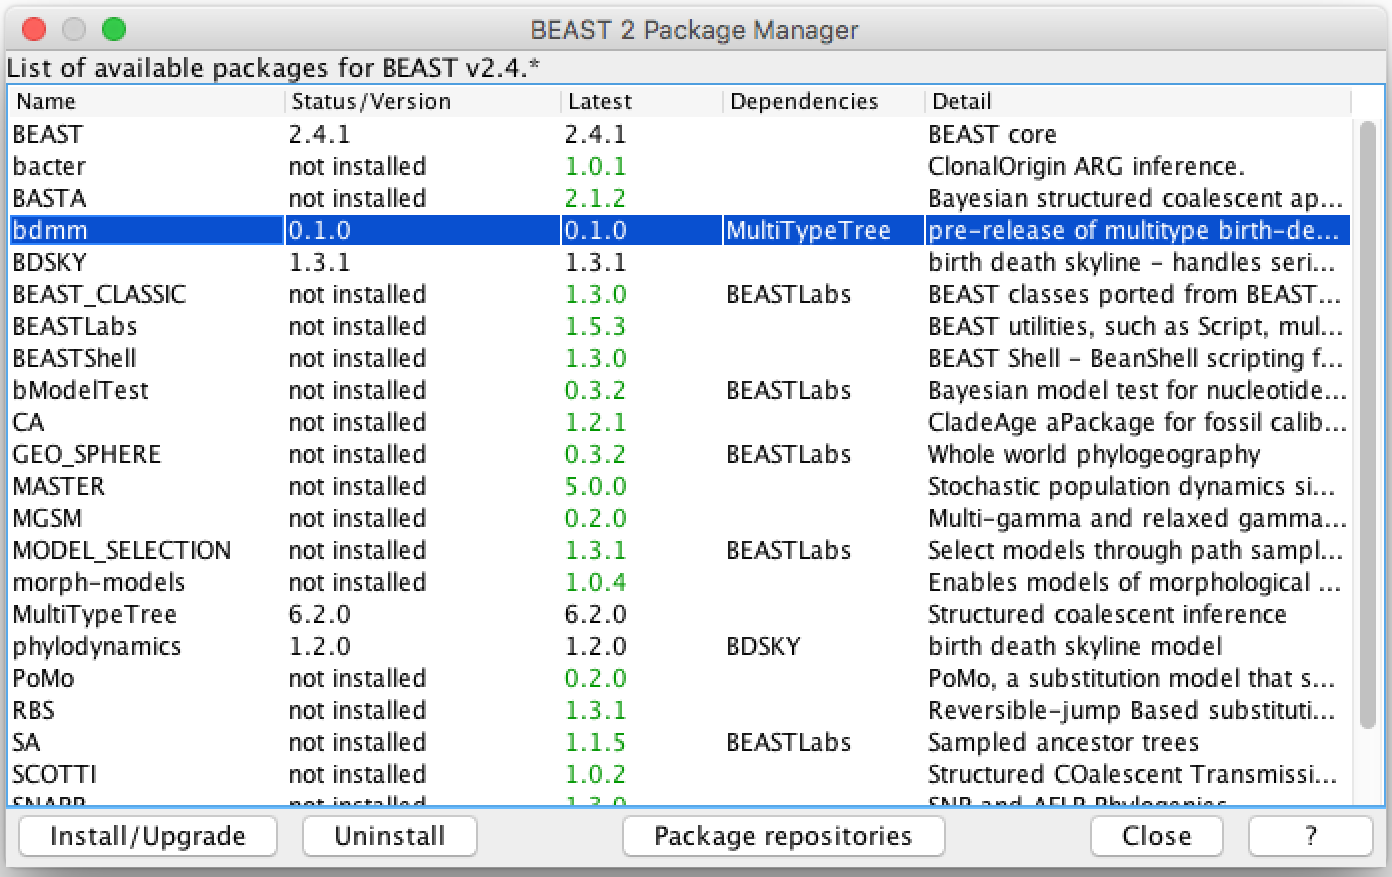
\includegraphics[width=0.750000\textwidth]{figures/1-install-bdmm.png}
    \caption{Install bdmm.}
    \label{fig:install-bdmm}
\end{figure}

Finally, \textbf{restart BEAUti.} The restart is necessary for the
packages to be successfully installed.

If you get an error message stating that you are missing a package on which  \lstinline!bdmm! depends, install that package manually using the package manager as done above, and \textbf{restart BEAUti} again.

\section{Setting up the analysis using
BEAUti}\label{setting-up-the-analysis-using-beauti}

\subsection{Loading the Template}\label{loading-the-template}

A BEAUTi template defines the basic structure and contents of your XML
configuration file. By default BEAUTi will construct an XML file with
standard uncoloured BEAST trees, however \lstinline!bdmm! uses coloured
trees which are defined in the \lstinline!MultiTypeTree! package. To use
the appropriate template for the configuration file, select
\lstinline!File > Template > MultiTypeBirthDeath!, as shown in Figure
\ref{fig:choose-bdmm}.

\begin{figure}
    \centering
    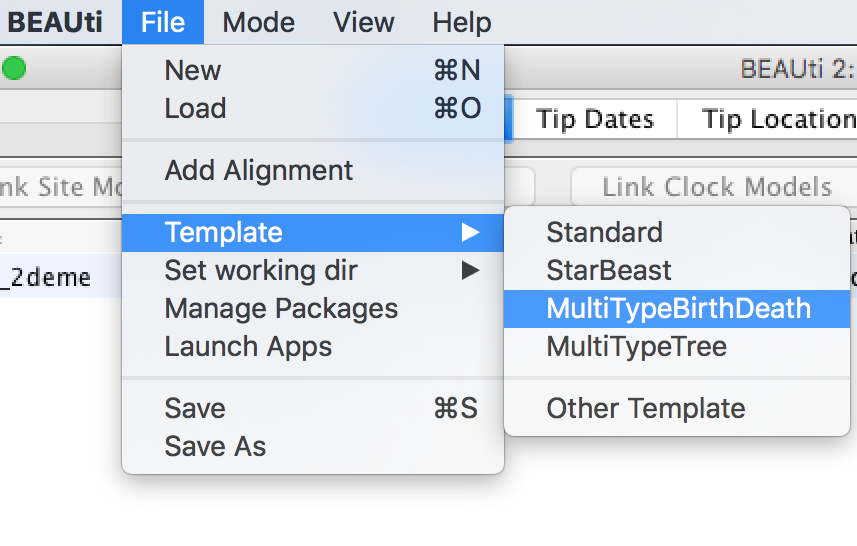
\includegraphics[width=1.000000\textwidth]{figures/2-choose-bdmm-template.png}
    \caption{Load the MultiTypeBirthDeath template.}
    \label{fig:choose-bdmm}
\end{figure}

\subsection{Loading the data}\label{loading-the-data}

Once the template is loaded, we can load in our example sequence data.
In our case, this data is stored in a FASTA file, the first few lines of
which look like this (the sequences have been truncated for better
readability):

\begin{lstlisting}
> EU856841_HongKong_2005.34246575
-----------GGGATAATTCTATTAACCATGAAGACTATCATTGCTTTGAGCTACATTT...
> EU856989_HongKong_2002.58356164
--CAAAAGCAGGGGATAATTCTATTAACCATGAAGACTATCATTGCTTTGAGCTACATTT...
> CY039495_HongKong_2004.5890411
------------------TTCTATTAACCATGAAGACTATCATTGCTTTGAGCTACATTC...
> EU856853_HongKong_2001.17808219
---------------------TATTAACCATGAAGACTATCATTGCTTTGAGCTACATTC...
> CY010084_NewZealand_2005.62739726
---------------------TATTAACCATGAAGACTATCATTGCTTTGAGCTACATTC...
> CY007387_NewZealand_2004.63287671
---------------------TATTAACCATGAAGACTATCATTGCTTTGAGCTACATTC...
> CY012432_NewZealand_2000.81643836
---------------------------CCATGAAGACTATCATTGCTTTGAGCTACATTT...
\end{lstlisting}

The lines beginning with ``\textgreater{}'' are labels for the sequences
immediately following. In general, these labels have no special format,
but in this file each label is an underscore-delimited triple. The first
element of each triple is the GenBank accession number of the sequence,
the second is the geographical region from which it was sampled, and the
third is the time at which it was sampled measured in calendar years or
fractions thereof.

In this tutorial we will be using the influenza sequence data which can
be found in the \lstinline!examples! folder of the
\lstinline!MultiTypeTree! package. To make it easier to find when
loading the alignment, you can optionally set the working directory of
BEAST2 to \lstinline!MultiTypeTree!. This will make BEAUTi open the
appropriate package folder when you look for the alignment. To set the
working directory, select
\lstinline!File > Set working dir > MultiTypeTree!, as shown in Figure
\ref{fig:working-dir}.

\begin{figure}
    \centering
    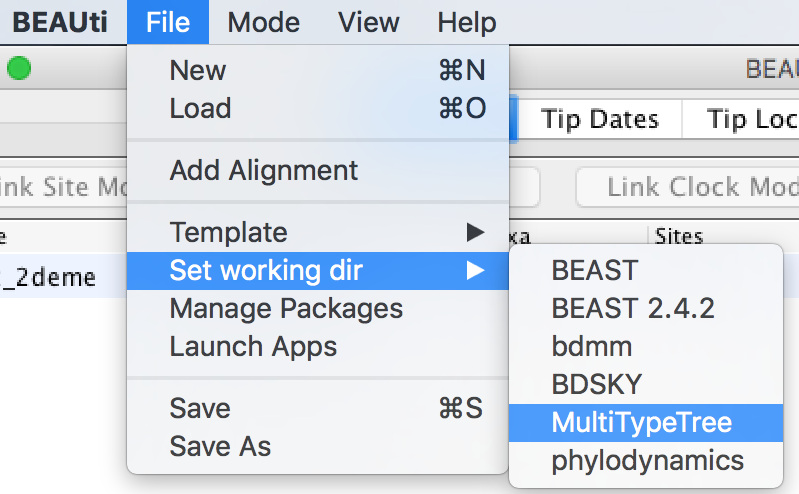
\includegraphics[width=1.000000\textwidth]{figures/3-set-working-dir.png}
    \caption{Optional step: set the working directory to MultiTypeTree.}
    \label{fig:working-dir}
\end{figure}

To load the file, select \lstinline!File > Add alignment!.

This will open a file selection dialog box. The example influenza
sequence data file is named \lstinline!h3n2_2deme.fna!. Assuming you
have followed the previous step to set the working directory, this can
be found in the \lstinline!examples/! directory shown when the file
selection dialog box appears. In case you have not followed the previous
step you will have to locate the folder containing the
\lstinline!MultiTypeTree! package and look for the \lstinline!examples/!
folder there.

Once the sequence file is loaded, your BEAUti screen should look similar
to what is shown in Figure \ref{fig:alignment}.

\begin{figure}
    \centering
    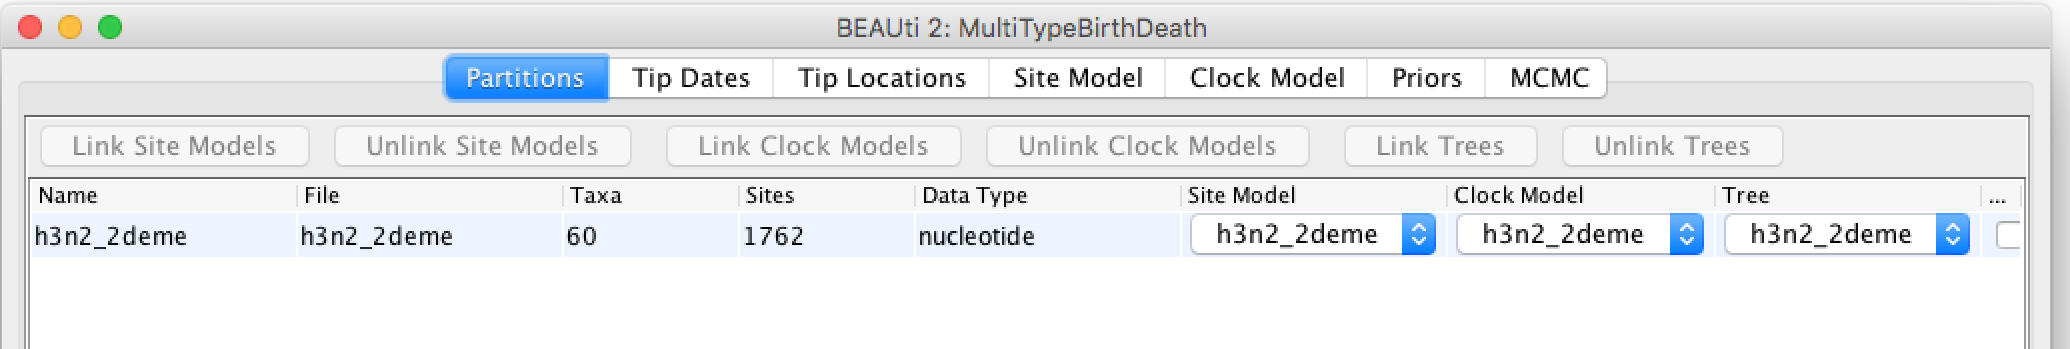
\includegraphics[width=1.000000\textwidth]{figures/4-alignment-loaded.png}
    \caption{The alignment loaded into BEAUti.}
    \label{fig:alignment}
\end{figure}

\subsection{Setting up dates}\label{setting-up-dates}

Once the data is loaded, the next step is to specify the times at which
the sequences were sampled:

\begin{enumerate}
\def\labelenumi{\arabic{enumi}.}

\item
  Select the \lstinline!Tip Dates! panel.
\item
  Check the \lstinline!Use tip dates! checkbox.
\item
  Click the \lstinline!Auto-configure! button at the top-right of the
  panel. This opens a dialog that allows sample times to be loaded from
  a file or inferred (guessed) from the sequence labels.
\item
  Because the times are included as the last element of the
  underscore-delimited sequence names, choose the
  \lstinline!use everything! radio button and select
  \lstinline!after last! from the drop-down menu. The default delimiter
  is already the underscore, so there is no need to change that.
\end{enumerate}

The date parsing setup will look as shown in Figure \ref{fig:tip-dates}.

\begin{figure}
    \centering
    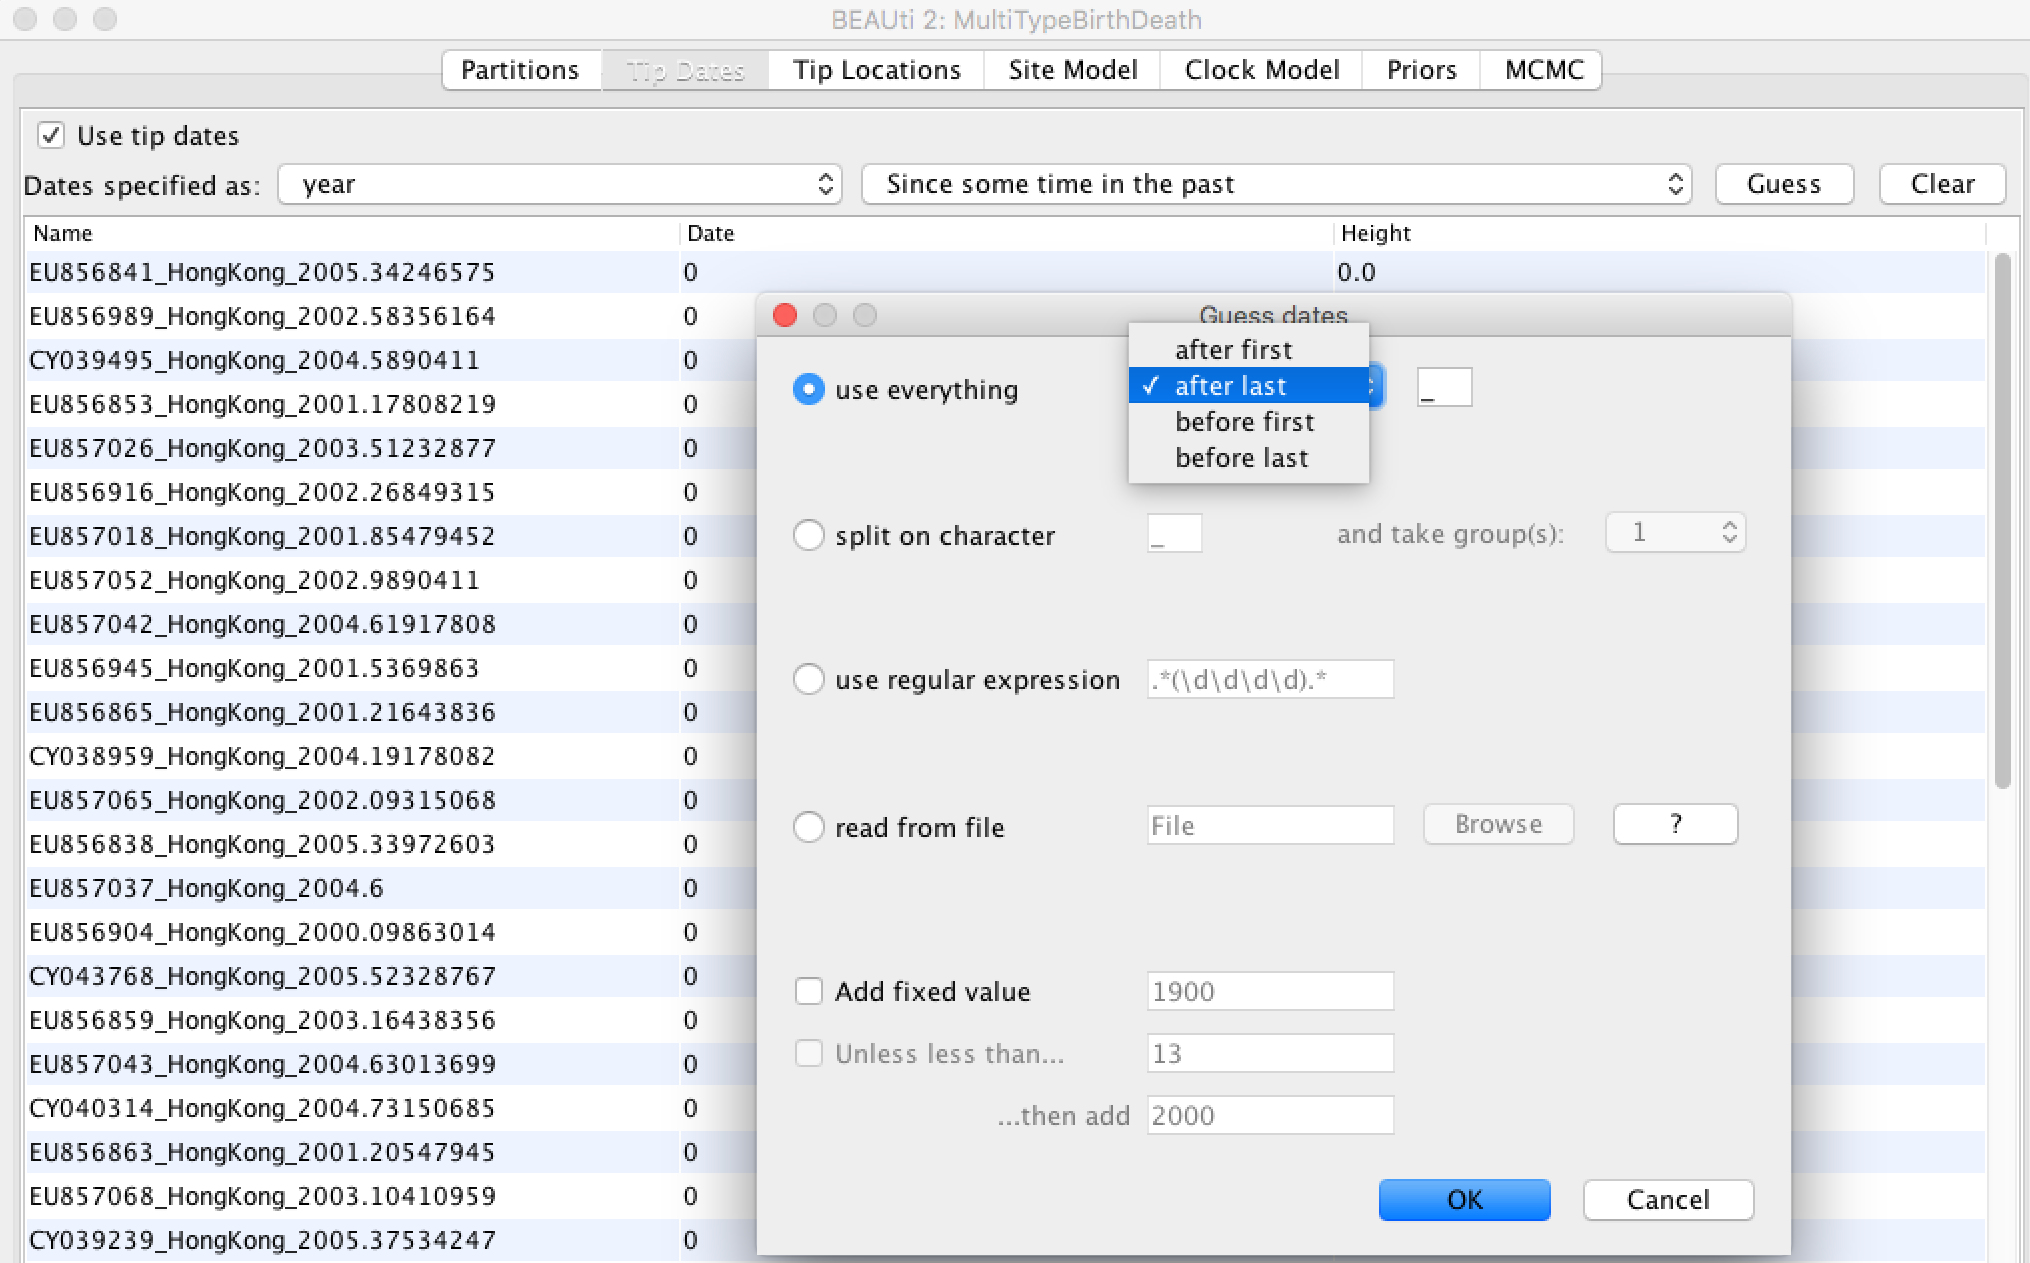
\includegraphics[width=0.750000\textwidth]{figures/5-tip-dates.png}
    \caption{Guessing the tip dates.}
    \label{fig:tip-dates}
\end{figure}

After clicking \lstinline!OK! you should find that the tip date table is
filled with times that match those in the sequence headers, and that the
last column of the table contains heights, i.e.~times before most recent
sample, calculated from the times. The BEAUTi panel should look as shown
in Figure \ref{fig:tip-dates}.

\begin{figure}
    \centering
    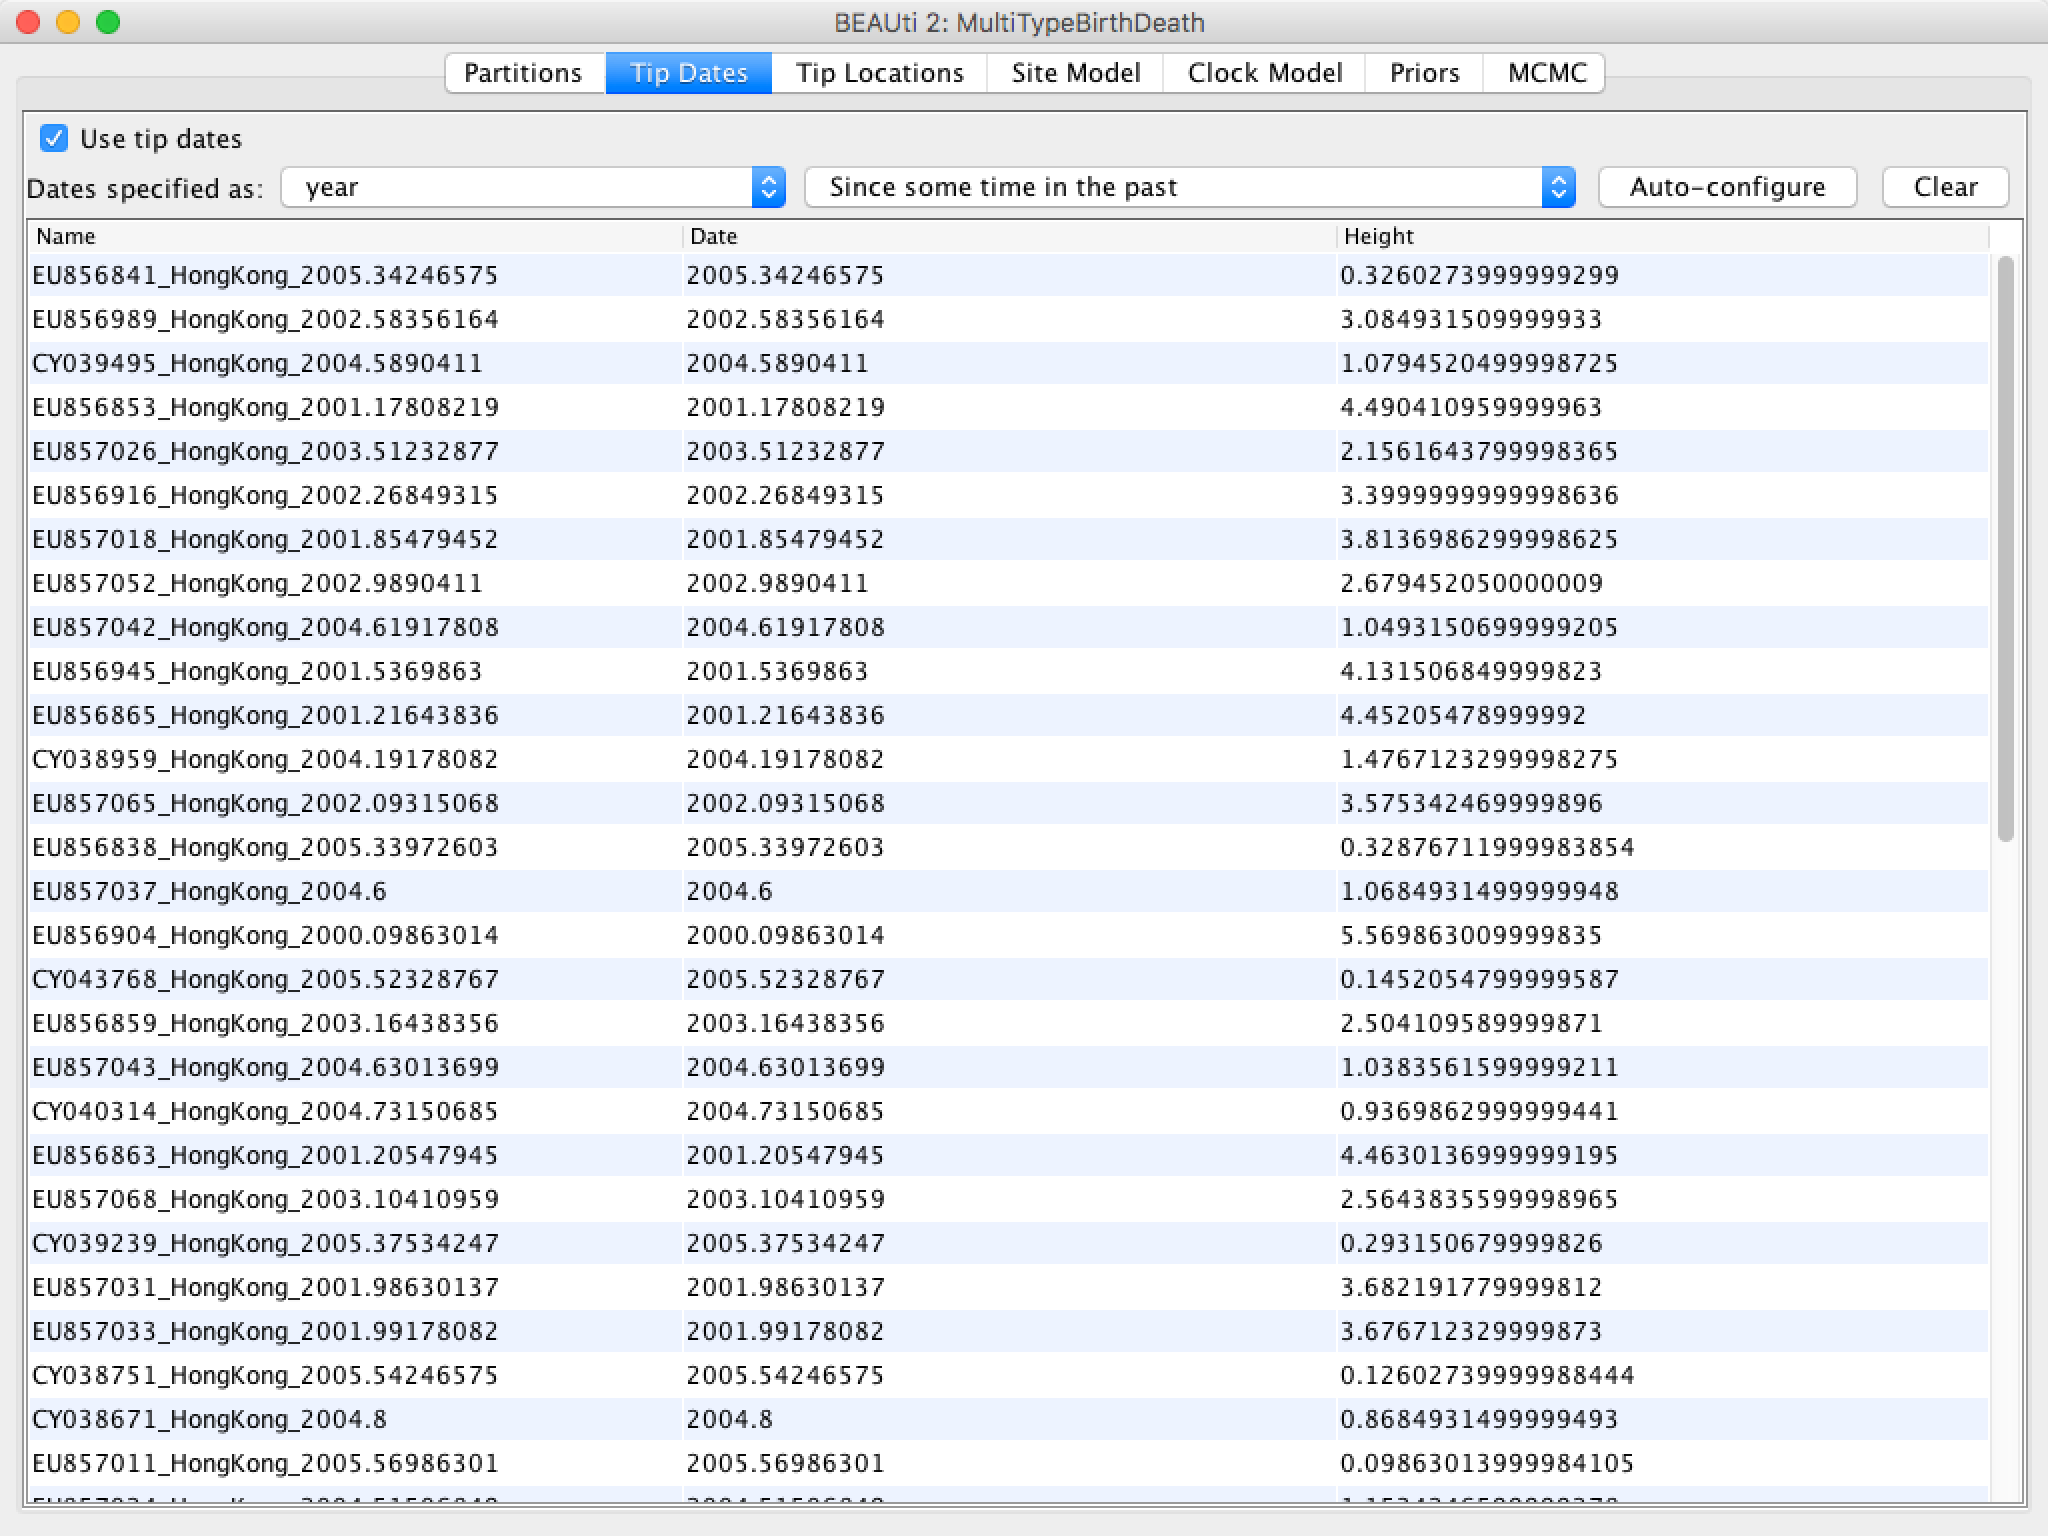
\includegraphics[width=1.000000\textwidth]{figures/6-tip-dates-set.png}
    \caption{Sampling dates as seen in BEAUti.}
    \label{fig:tip-dates-set}
\end{figure}

\subsection{Setting up locations}\label{setting-up-locations}

Now that we've specified the sampling times, we move on to specifying
the sampling locations. To do this, we follow a very similar set of
steps to those we used to set the sample times:

\begin{enumerate}
\def\labelenumi{\arabic{enumi}.}

\item
  Select the \lstinline!Tip Locations! panel. You'll find that the
  locations are already filled with a single default value --
  \lstinline!NOT_SET!.
\item
  Click the \lstinline!Guess! button at the top-right of the panel. This
  opens the same dialog that we saw in the previous section when setting
  up the dates.
\item
  The locations are included as the second element of the
  underscore-delimited sequence names. Therefore we choose the
  \lstinline!split on character! radio button and select group
  \lstinline!2! from the drop-down menu. Note again that the underscore
  character is already chosen as the delimiter.
\end{enumerate}

The location parsing setup will look as shown in Figure
\ref{fig:tip-types}.

\begin{figure}
    \centering
    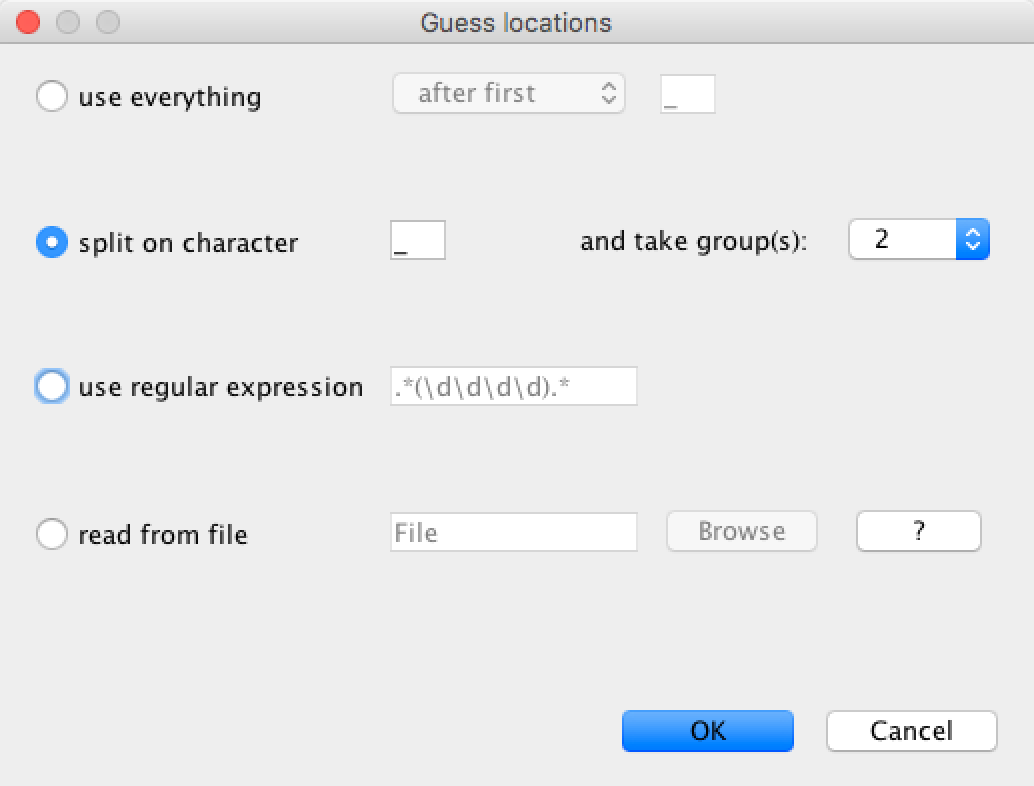
\includegraphics[width=0.750000\textwidth]{figures/7-tip-types.png}
    \caption{Guessing the locations.}
    \label{fig:tip-types}
\end{figure}

After clicking \lstinline!OK! you should find that the tip location
table is filled with locations that match those in the sequence titles.
The BEAUTi panel should look as shown in Figure \ref{fig:tip-types-set}.

\begin{figure}
    \centering
    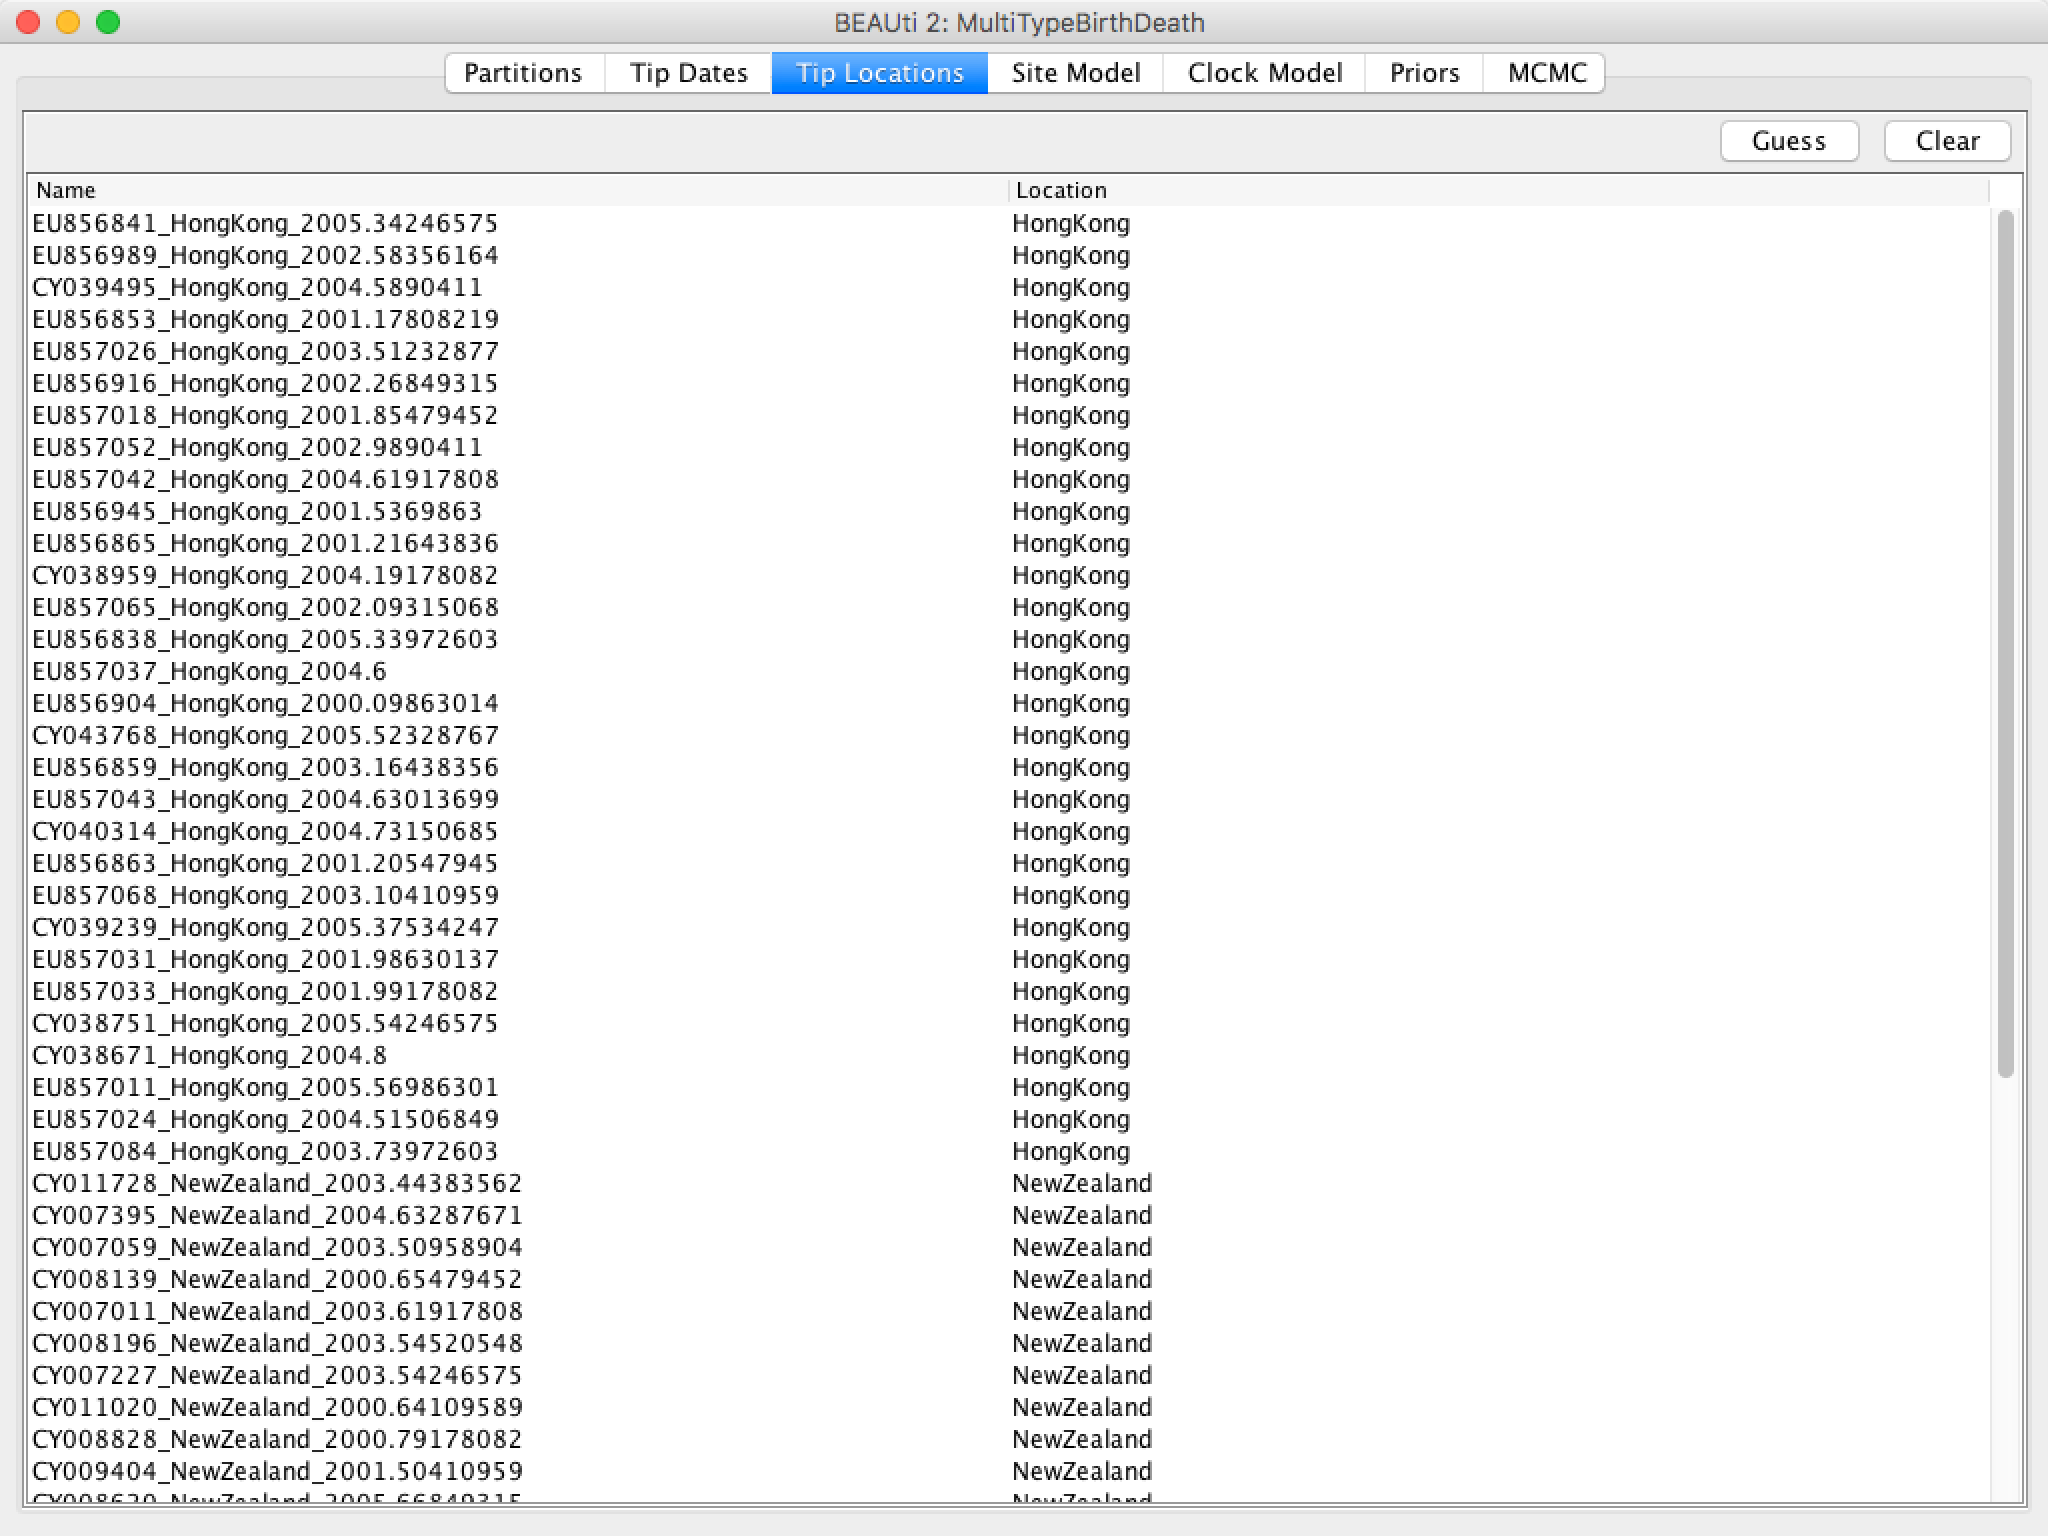
\includegraphics[width=1.000000\textwidth]{figures/8-tip-types-set.png}
    \caption{The locations in BEAUti.}
    \label{fig:tip-types-set}
\end{figure}

\subsection{Setting the substitution
model}\label{setting-the-substitution-model}

For this analysis, we will use the HKY substitution model with 4 gamma
categories and estimated base frequencies. To configure this in BEAUti,
switch to the \lstinline!Site Model! panel. First, we need to set up the
rate category count. To approximate the continuous gamma rate
distribution BEAST2 uses the discrete gamma distribution, where sites
are divided into k equally probable rate categories. In general, 4-6
categories work well for most datasets, while having more categories
involve a lot of computation at little precision gain, so we set the
\lstinline!Gamma category count! to 4. We would also like to estimate
the \lstinline!Shape! parameter, which describes the shape of the
continuous gamma distribution we approximate. To do so, we need to set
it to a non-zero value (e.g.~the default 1.0) and tick the
\lstinline!estimate! checkbox. While the gamma categories account for
rate variation, allowing some sites to have an evolutionary rate of 0
can improve fit to real data. To speed up the analysis we will fix this
to the actual proportion of invariant sites we have in our alignment,
which is 0.867.

Next, to set up the substitution model, select \lstinline!HKY! from the
drop-down menu (the default option is \lstinline!JC69!). We would like
to estimate the kappa parameter of HKY, so we leave the
\lstinline!Kappa! at the default value of 2.0 and leave the
\lstinline!estimate! checkbox checked. We would also like to estimate
nucleotide frequencies, so we leave the \lstinline!Frequencies!
parameter at the default value (\lstinline!Estimated!). The BEAUti panel
should now look as shown in Figure \ref{fig:site-model}.

\begin{figure}
    \centering
    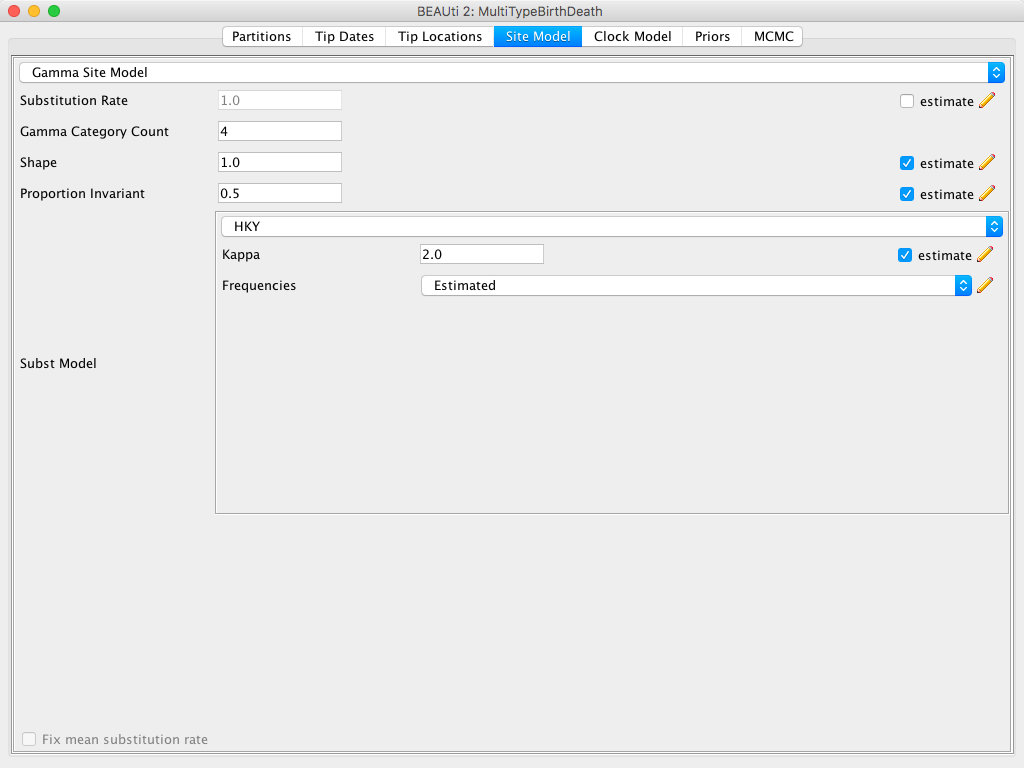
\includegraphics[width=1.000000\textwidth]{figures/9-sitemodel.png}
    \caption{Setup of the site model.}
    \label{fig:site-model}
\end{figure}

Note that the \lstinline!Substitution rate! defined on this panel should
not be estimated - we use the \lstinline!Clock rate! defined in the
\lstinline!Clock Model! panel to determine the average per unit time
rate of sequence evolution. This way, the \lstinline!Substitution rate!
is not actually a rate, but rather a rate multiplier that we fix to 1 to
allow parameter identifiability.

\subsection{Setting the clock model}\label{setting-the-clock-model}

To speed up the analysis we will assume a strict clock for this small
dataset. dataset. However, the selection of a clock model for a
different, real analysis should not be taken lightly. Since our
alignment contains sequences sampled at different times and those times
are measured in years, we must use a clock rate expressed in units of
expected substitutions per site per year. Usually the precise value is
unknown and so the default behaviour of BEAUti is to assume this rate
has to be estimated. To speed up mixing we set the starting value of the
\lstinline!Clock rate! to 0.005, which we know from research to be much
closer to the truth than the default value of 1. The
\lstinline!Clock Model! panel should now look as shown in Figure
\ref{fig:strict-clock}.

\begin{figure}
    \centering
    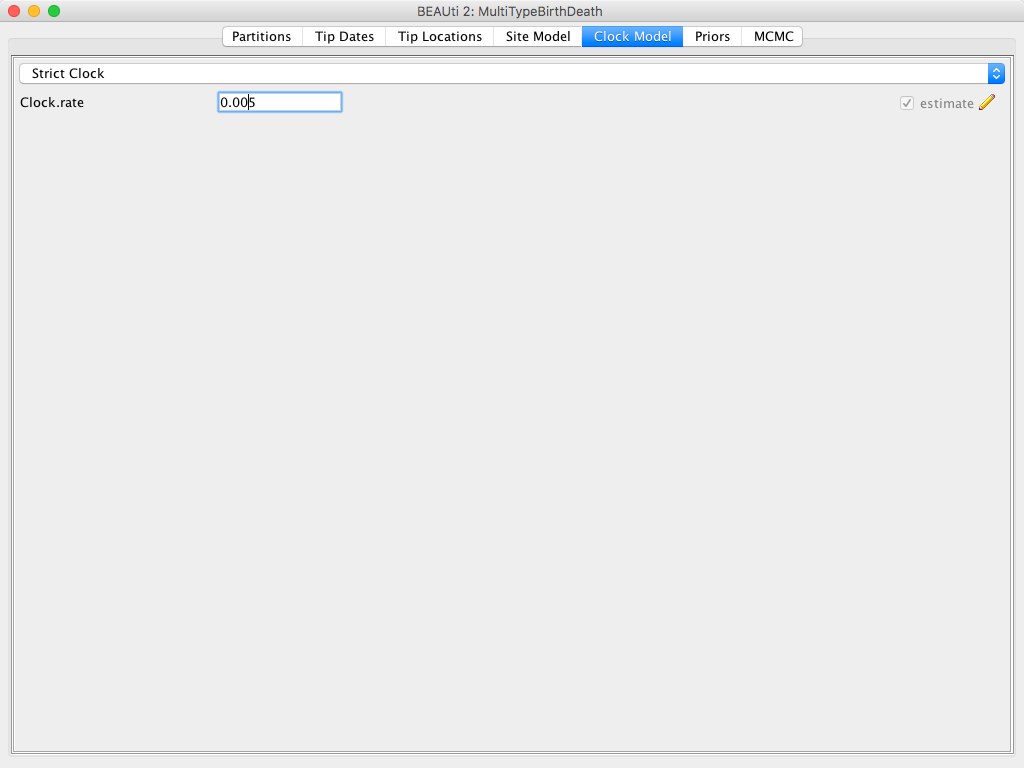
\includegraphics[width=1.000000\textwidth]{figures/10-strict-clock.png}
    \caption{Fix the clock rate to speed up mixing.}
    \label{fig:strict-clock}
\end{figure}

\subsection{Adjusting Priors}\label{adjusting-priors}

\subsubsection{\texorpdfstring{Setting up the \texttt{bdmm} tree
prior}{Setting up the bdmm tree prior}}\label{setting-up-the-bdmm-tree-prior}

\lstinline!bdmm! defines a prior on the multi-type tree distribution.
Thus it is particularly important for the analysis that we properly set
up the priors. First, let's talk about the values that need to be set on
the \lstinline!Priors! panel. The first panel that you see at the top is
the tree prior.

\lstinline!bdmm! is a model that can be used to explain data that is
clearly divided into separate partitions, or demes. The demes can be
geographical locations, as in our example, but the sequences can also be
separated through other means than that, e.g.~by a specific drug
resistance mutation (strains can develop/lose drug resistance and thus
move between demes, but can not transfer between demes otherwise), or
location in the body (for example, for localised infections caused by
the same agent). In this dataset we have strains from 2 different
locations, New Zealand and Hong Kong, so the \lstinline!Number of demes!
should be set to 2, which also is the default value. Next,
\lstinline!bdmm! lets you estimate the
\lstinline!Reproduction number per type! and the
\lstinline!BecomeUninfectiousRate per type!. This will let us see the
differences in reproduction fitness and speed of recovery between the
two locations, so we leave the \lstinline!estimate! checkboxes checked.
We can leave the starting values at default as it will not influence the
inference a lot.

The next important thing one should take care of is setting the sampling
proportions appropriately. In general, the trees that we build go back
in time much further than the first sample that we have. If we set the
same sampling proportion for the whole time period from our estimated
tree origin to the time of the last sample, we will most likely run into
trouble, as \lstinline!bdmm! will try to produce a tree that has the
same sampling proportion for the whole time, but no samples in the past
and a lot of samples towards the present. In order to remove that bias
from the trees, we need to make sure that we only have non-zero sampling
starting from the first sample date (unless we know that there really
weren't any related cases before the first sampled case). To do so,
let's look at the \lstinline!SamplingProportion per type! field. You
will see that it has 4 values, which correspond to two values per type,
lets call them {[}v1,v2,v3,v4{]}. v1 and v2 are the values for the first
and second time interval for the first deme, and v3 and v4 are the
values for the second deme. Thus, to do what we want we need to set the
values v1 and v3 to zero. Because BEAST2 will use scalers to sample new
values for the sampling proportions, the values which we set to 0 will
remain so. Next, we also need to set the
\lstinline!Sampling change time! to the time slightly before the first
sample. If we look back at the \lstinline!Tip dates! panel, we can see
that our oldest sample is the one labelled as
\lstinline!EU856904_HongKong_2000.09863014!, for which the height, or
the length of time from the first sample and the last, is 5.569863. We
set the sampling change time in time units from the most recent sample
and we need to make sure we include the first sample, thus we set the
\lstinline!Sampling change time! to 5.57, which is the height of the
first sample rounded slightly up (and confirm the change with ENTER).
The final setup of the tree prior can be seen in Figure
\ref{fig:tree-prior}.

\begin{figure}
    \centering
    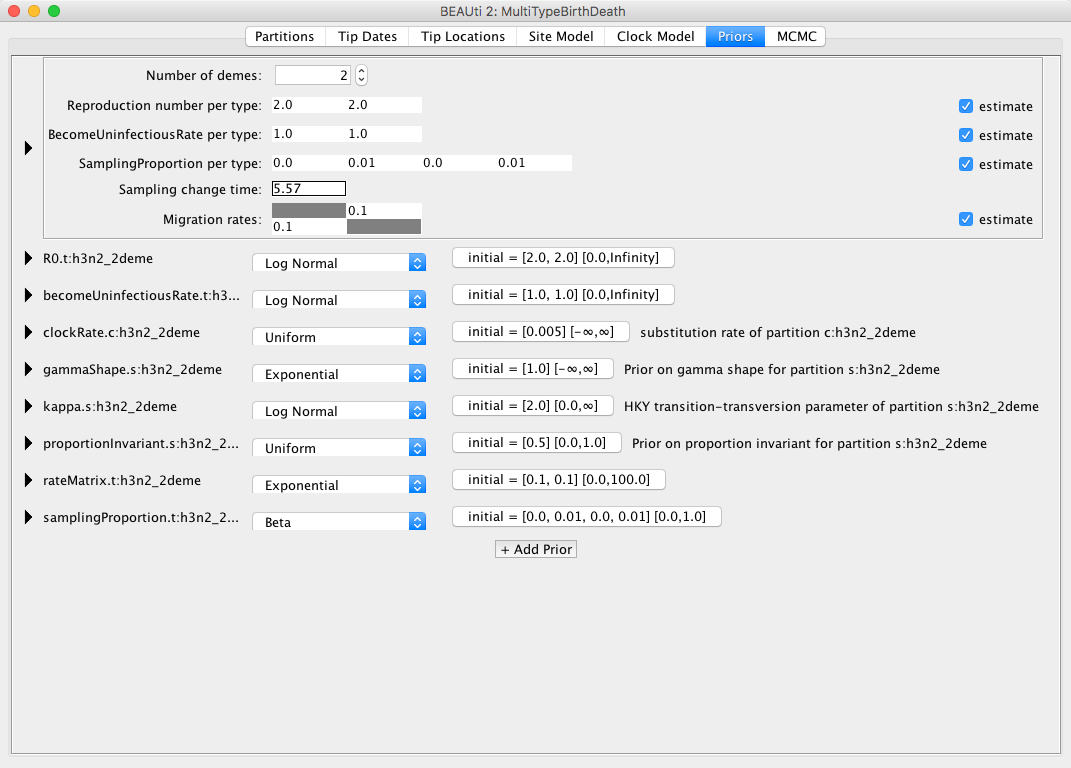
\includegraphics[width=1.000000\textwidth]{figures/11-tree-prior.png}
    \caption{Set the change time for the sampling proportion so it is zero before the time of the first sample.}
    \label{fig:tree-prior}
\end{figure}

\paragraph{What if you have more
demes?}\label{what-if-you-have-more-demes}

First things first, for an analysis with more demes you need to set the
\lstinline!Number of demes! to the appropriate value, e.g.~N, that
actually corresponds to the number of demes in the dataset. When you do
that, the dimensions of the parameters \lstinline!Reproduction number!,
\lstinline!BecomeUninfectiousRate!, \lstinline!SamplingProportion! and
\lstinline!Migration rates! will change. The
\lstinline!Reproduction number! and the
\lstinline!BecomeUninfectiousRate! will have as many values as you have
demes. The dimensionality of the \lstinline!SamplingProportion! will be
the number of demes times 2, so in case you have 4 demes your sampling
proportion will need 8 values. You can view this parameter as a matrix
of 2 x N values, which is flattened by row. The first column reflects
the sampling rate before first sample and all of the values in it should
be set to 0. The \lstinline!Sampling change time! obviously does not
change dimensionality, but has to be set to the appropriate time for
your dataset. Finally, the \lstinline!Migration rates! will have N * (N
- 1) entries. As one can imagine, the matrix should have the dimensions
of N * N, however since there is no migration from a deme to itself
(values on the diagonal of the matrix), we subtract N values from the
dimensionality, getting N * (N - 1).

\subsubsection{Setting up other priors}\label{setting-up-other-priors}

By default, BEAST2 provides you with a prior distribution for each of
the parameters of your model. This is done because otherwise BEAUTi will
have a hard time displaying all of the parameters without any settings
provided. Unfortunately, this means that some priors are very generic,
and, moreover, some priors are in fact, improper -- the distribution
does not integrate to one. This means that while the default setup might
work and the runs will eventually mix, it can happen that the values are
meaningless.

So, let us go through the important parameters and set priors according
to the information we have about our dataset. The first important
parameter is R0. In epidemiology, the basic reproduction number, R0, of
an infection is the number of secondary cases one case generates on
average over the course of its infectious period, in an otherwise
uninfected population. Even though we do not have any information on R0
in the particular outbreak, infections rarely have R0 \textgreater{} 10,
so we can set an upper limit on the sampled values. To do so, in the
line denoted \lstinline!R0.t:h3n2_2deme! click the button captioned
\lstinline!initial = [2.0, 2.0] [0.0, Infinity]! to get a pop up
settings window (see Figure \ref{fig:R0-prior}), where you can set the
upper value. Other than that, the current prior sets ther median value
of the distribution to e0 = 1, which will fit the endemic case of
influenza.

\begin{figure}
    \centering
    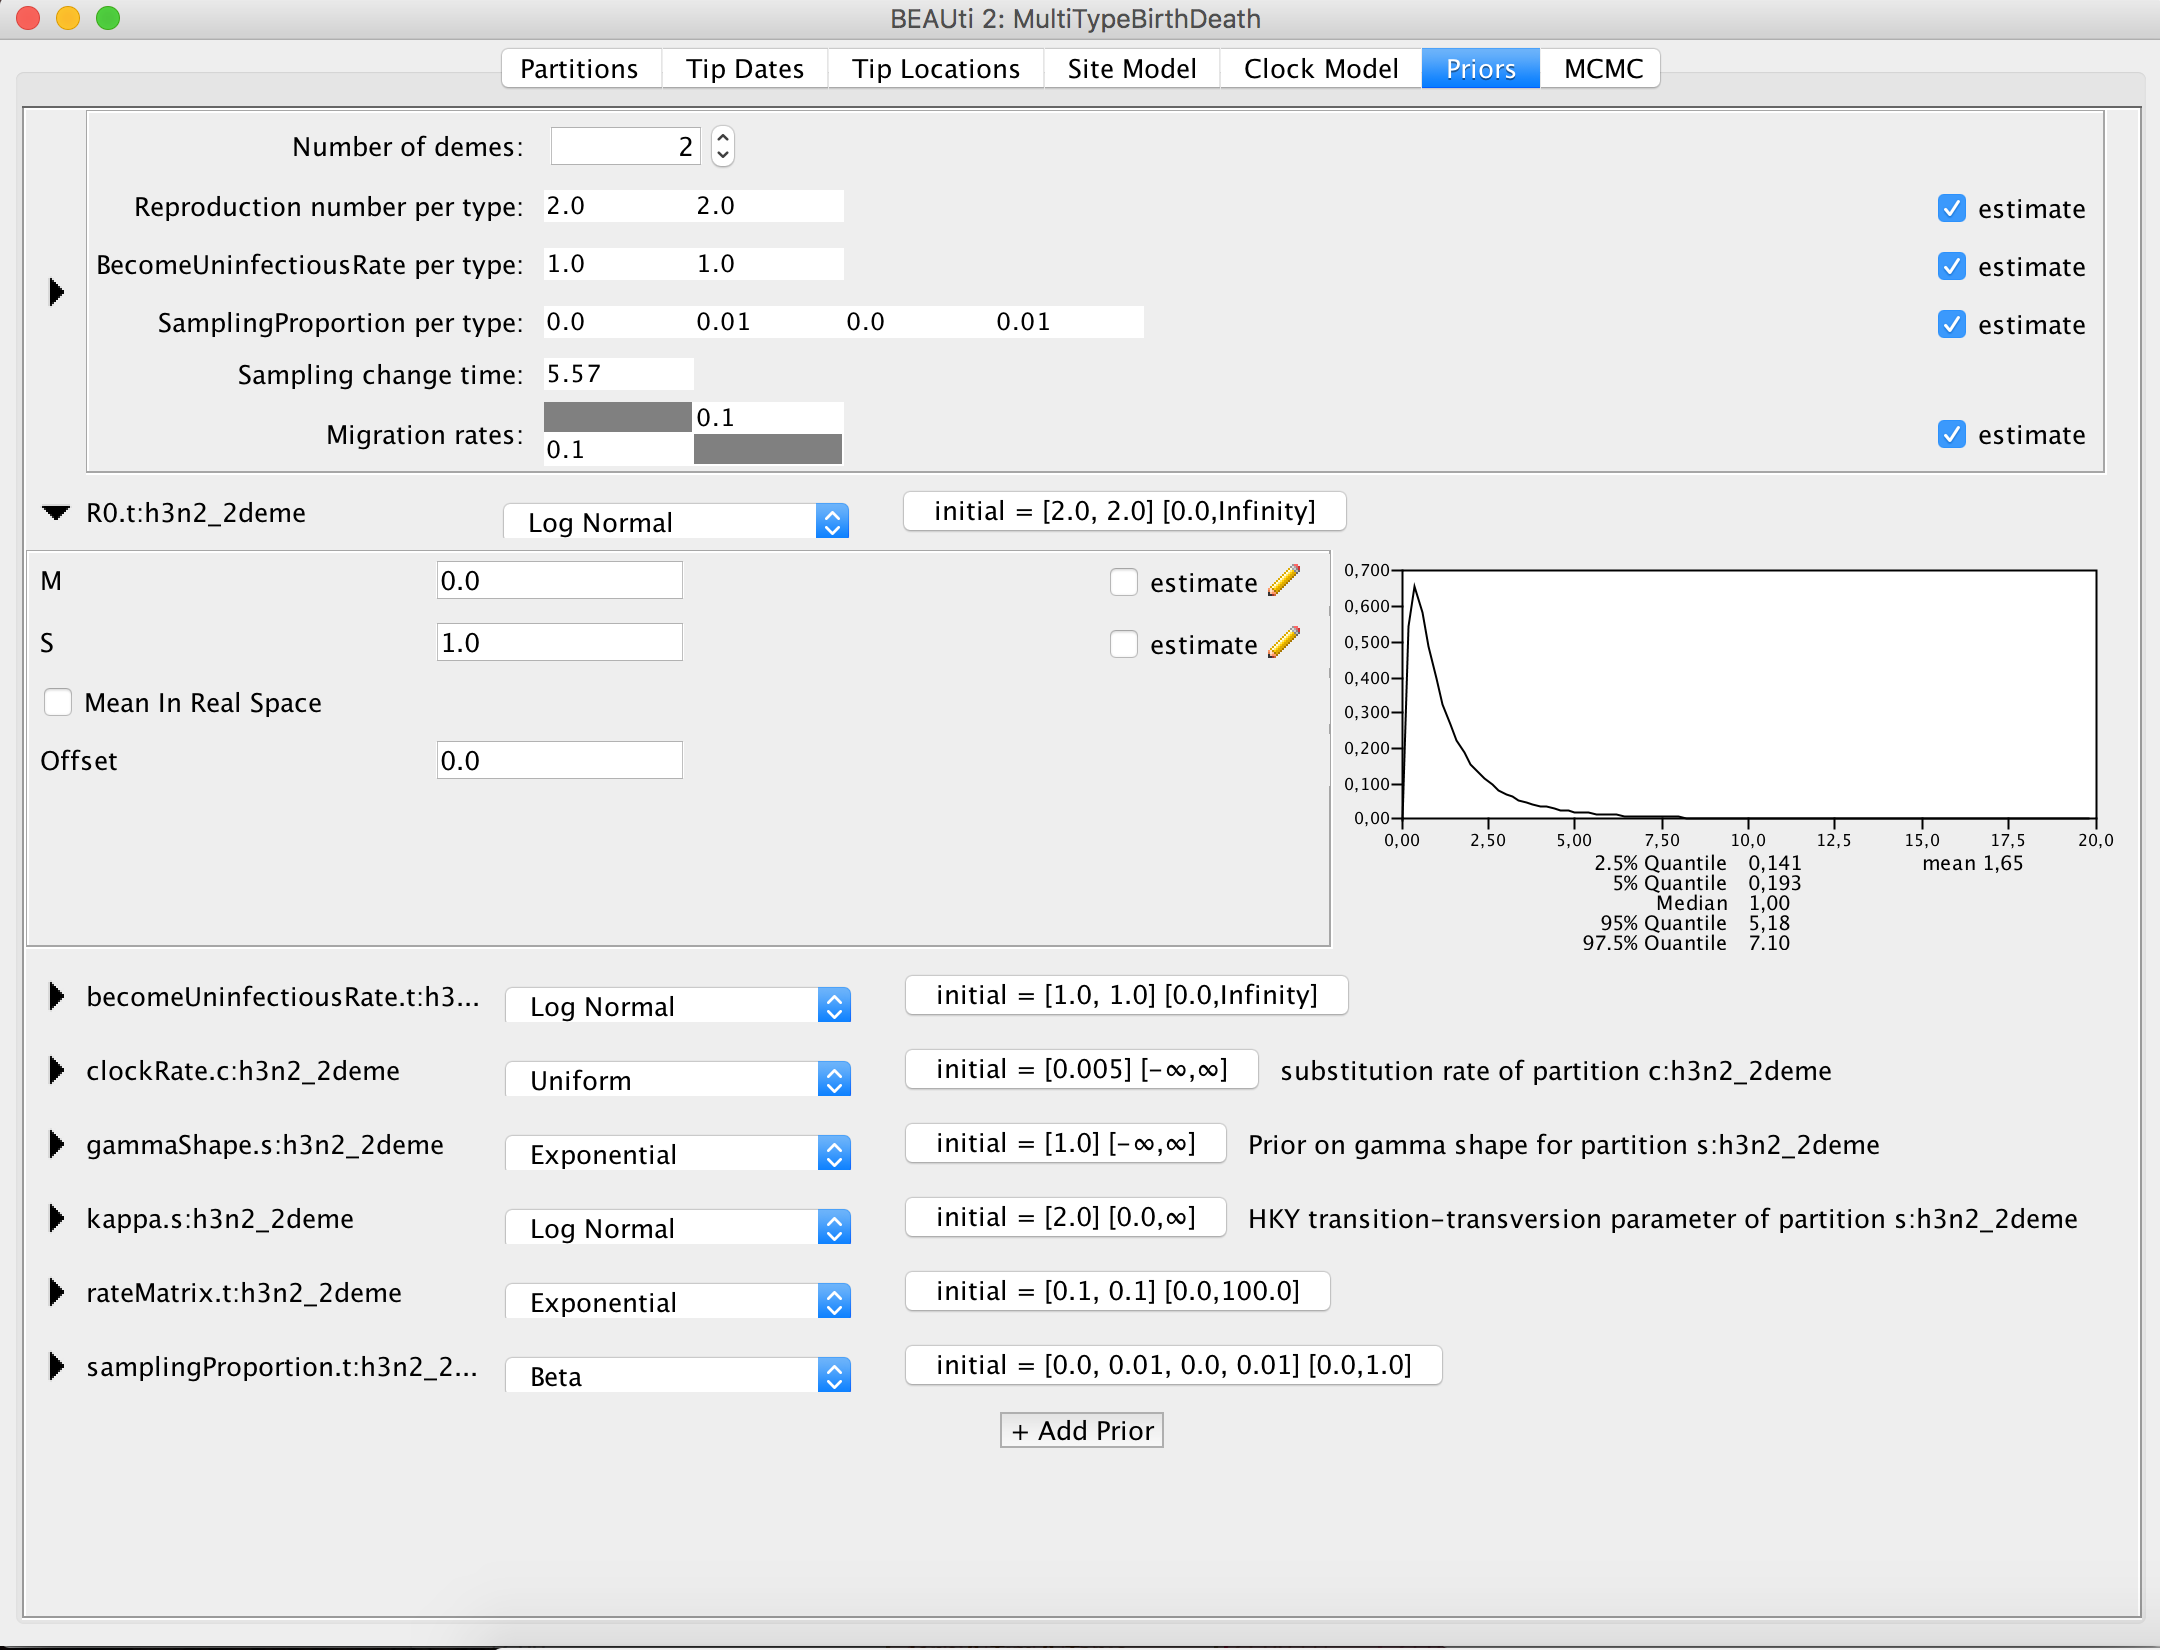
\includegraphics[width=1.000000\textwidth]{figures/12-R0-prior.png}
    \caption{Set the prior for the R<sub>0</sub>.}
    \label{fig:R0-prior}
\end{figure}

Next, we should adjust the prior for the rate of clearing the infection,
which is labelled as \lstinline!becomeUninfectiousRate.t:h3n2_2deme!.
The value of the rate, say x, is the reciprocal of the average time a
person with influenza is infectious, 1/x. From what we know about
influenza we can say that an average infection lasts for about a week,
however we would not want to impose too strong of a prior on this
parameter. Let us change the distribution for this parameter to a
\lstinline!LogNormal! and tick the \lstinline!Mean in Real Space!
checkbox to make the setting easier. So, for a mean time of recovery of
7 days we need to set the mean of our distribution to 365/7
$ \approx $ 52.14 (or to 52 for simplicity). Bear in mind
that our time units are years, so we can not just set the rate to 1/7.
This prior will ensure that we mainly sample realistic parameter values,
but still gives BEAST2 quite a lot of freedom to go to extreme values if
need be, as the 95\% highest density interval for the prior is {[}4.44,
224{]}, or {[}1.63, 82.21{]} infectious days. You can see the setup in
Figure \ref{fig:bUR-prior}.

\begin{figure}
    \centering
    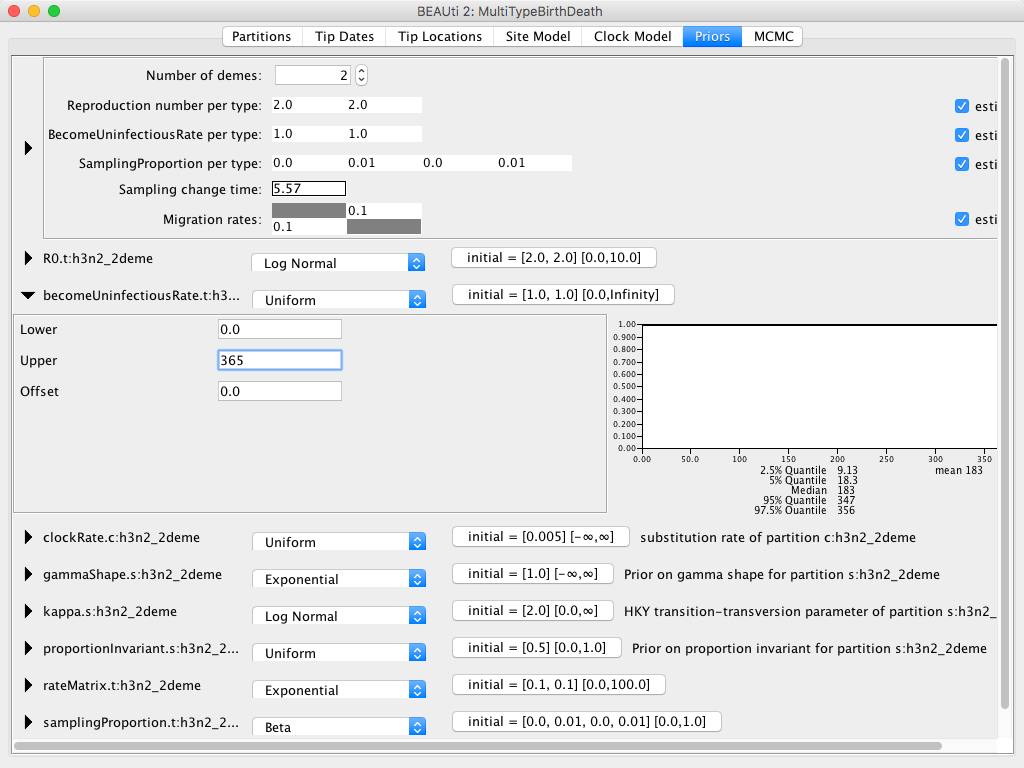
\includegraphics[width=1.000000\textwidth]{figures/13-bUR-prior.png}
    \caption{Set the prior for the rate of recovery.}
    \label{fig:bUR-prior}
\end{figure}

We will also set the prior for the clock rate to a distribution that is
in accordance with what we know about RNA viruses, which is that in
general their mean substitution rate is around $ \approx $
10$^{-3}$. We shall set the distribution for
\lstinline!clockRate.c:h3n2_2deme! to \lstinline!Log Normal! with the
mean of 0.001, with the \lstinline!Mean in Real Space! checkbox checked.
We will leave the \lstinline!S! parameter (standard deviation) at the
default value of 1.25 to allow BEAST2 a lot of freedom in case it is
necessary. The appropriate prior setup can be seen in Figure
\ref{fig:clock-rate-prior}.

\begin{figure}
    \centering
    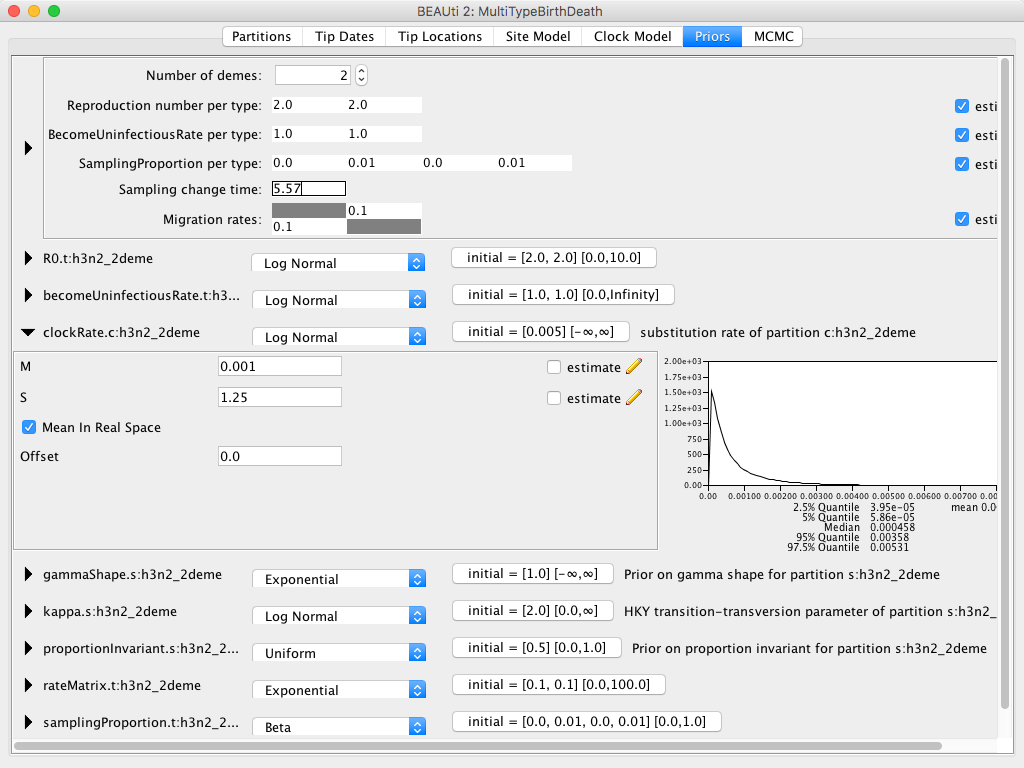
\includegraphics[width=1.000000\textwidth]{figures/14-clock-rate-prior.png}
    \caption{Set the prior for the clock rate.}
    \label{fig:clock-rate-prior}
\end{figure}

Lastly, we will set the sampling proportion prior to a more narrow
distribution peaked around the very low values, as influenza spreads
easily, but only few people actually get sampled. Taking into account
that we are also using a thinned-down version of the dataset, we can use
a diffuse prior with the mean around 10-3. The default prior for the
sampling proportion is a \lstinline!Beta! distribution, which is only
defined between 0 and 1, making it a natural choice for proportions.
Here, however, we will use a \lstinline!Log Normal! prior, with the mean
\lstinline!M! at 10-3 and the standard deviation \lstinline!S! at 1.25
to allow a lot of variance. Once again we need to check that the
\lstinline!Mean in Real Space! checkbox is checked, and since the
\lstinline!Log Normal! distribution is defined outside the range of
{[}0, 1{]} we also need to check that the \lstinline!Lower! and
\lstinline!Upper! limits are set accordingly. You can see the sampling
prior setup in Figure \ref{fig:samplingProportion-prior}

\begin{figure}
    \centering
    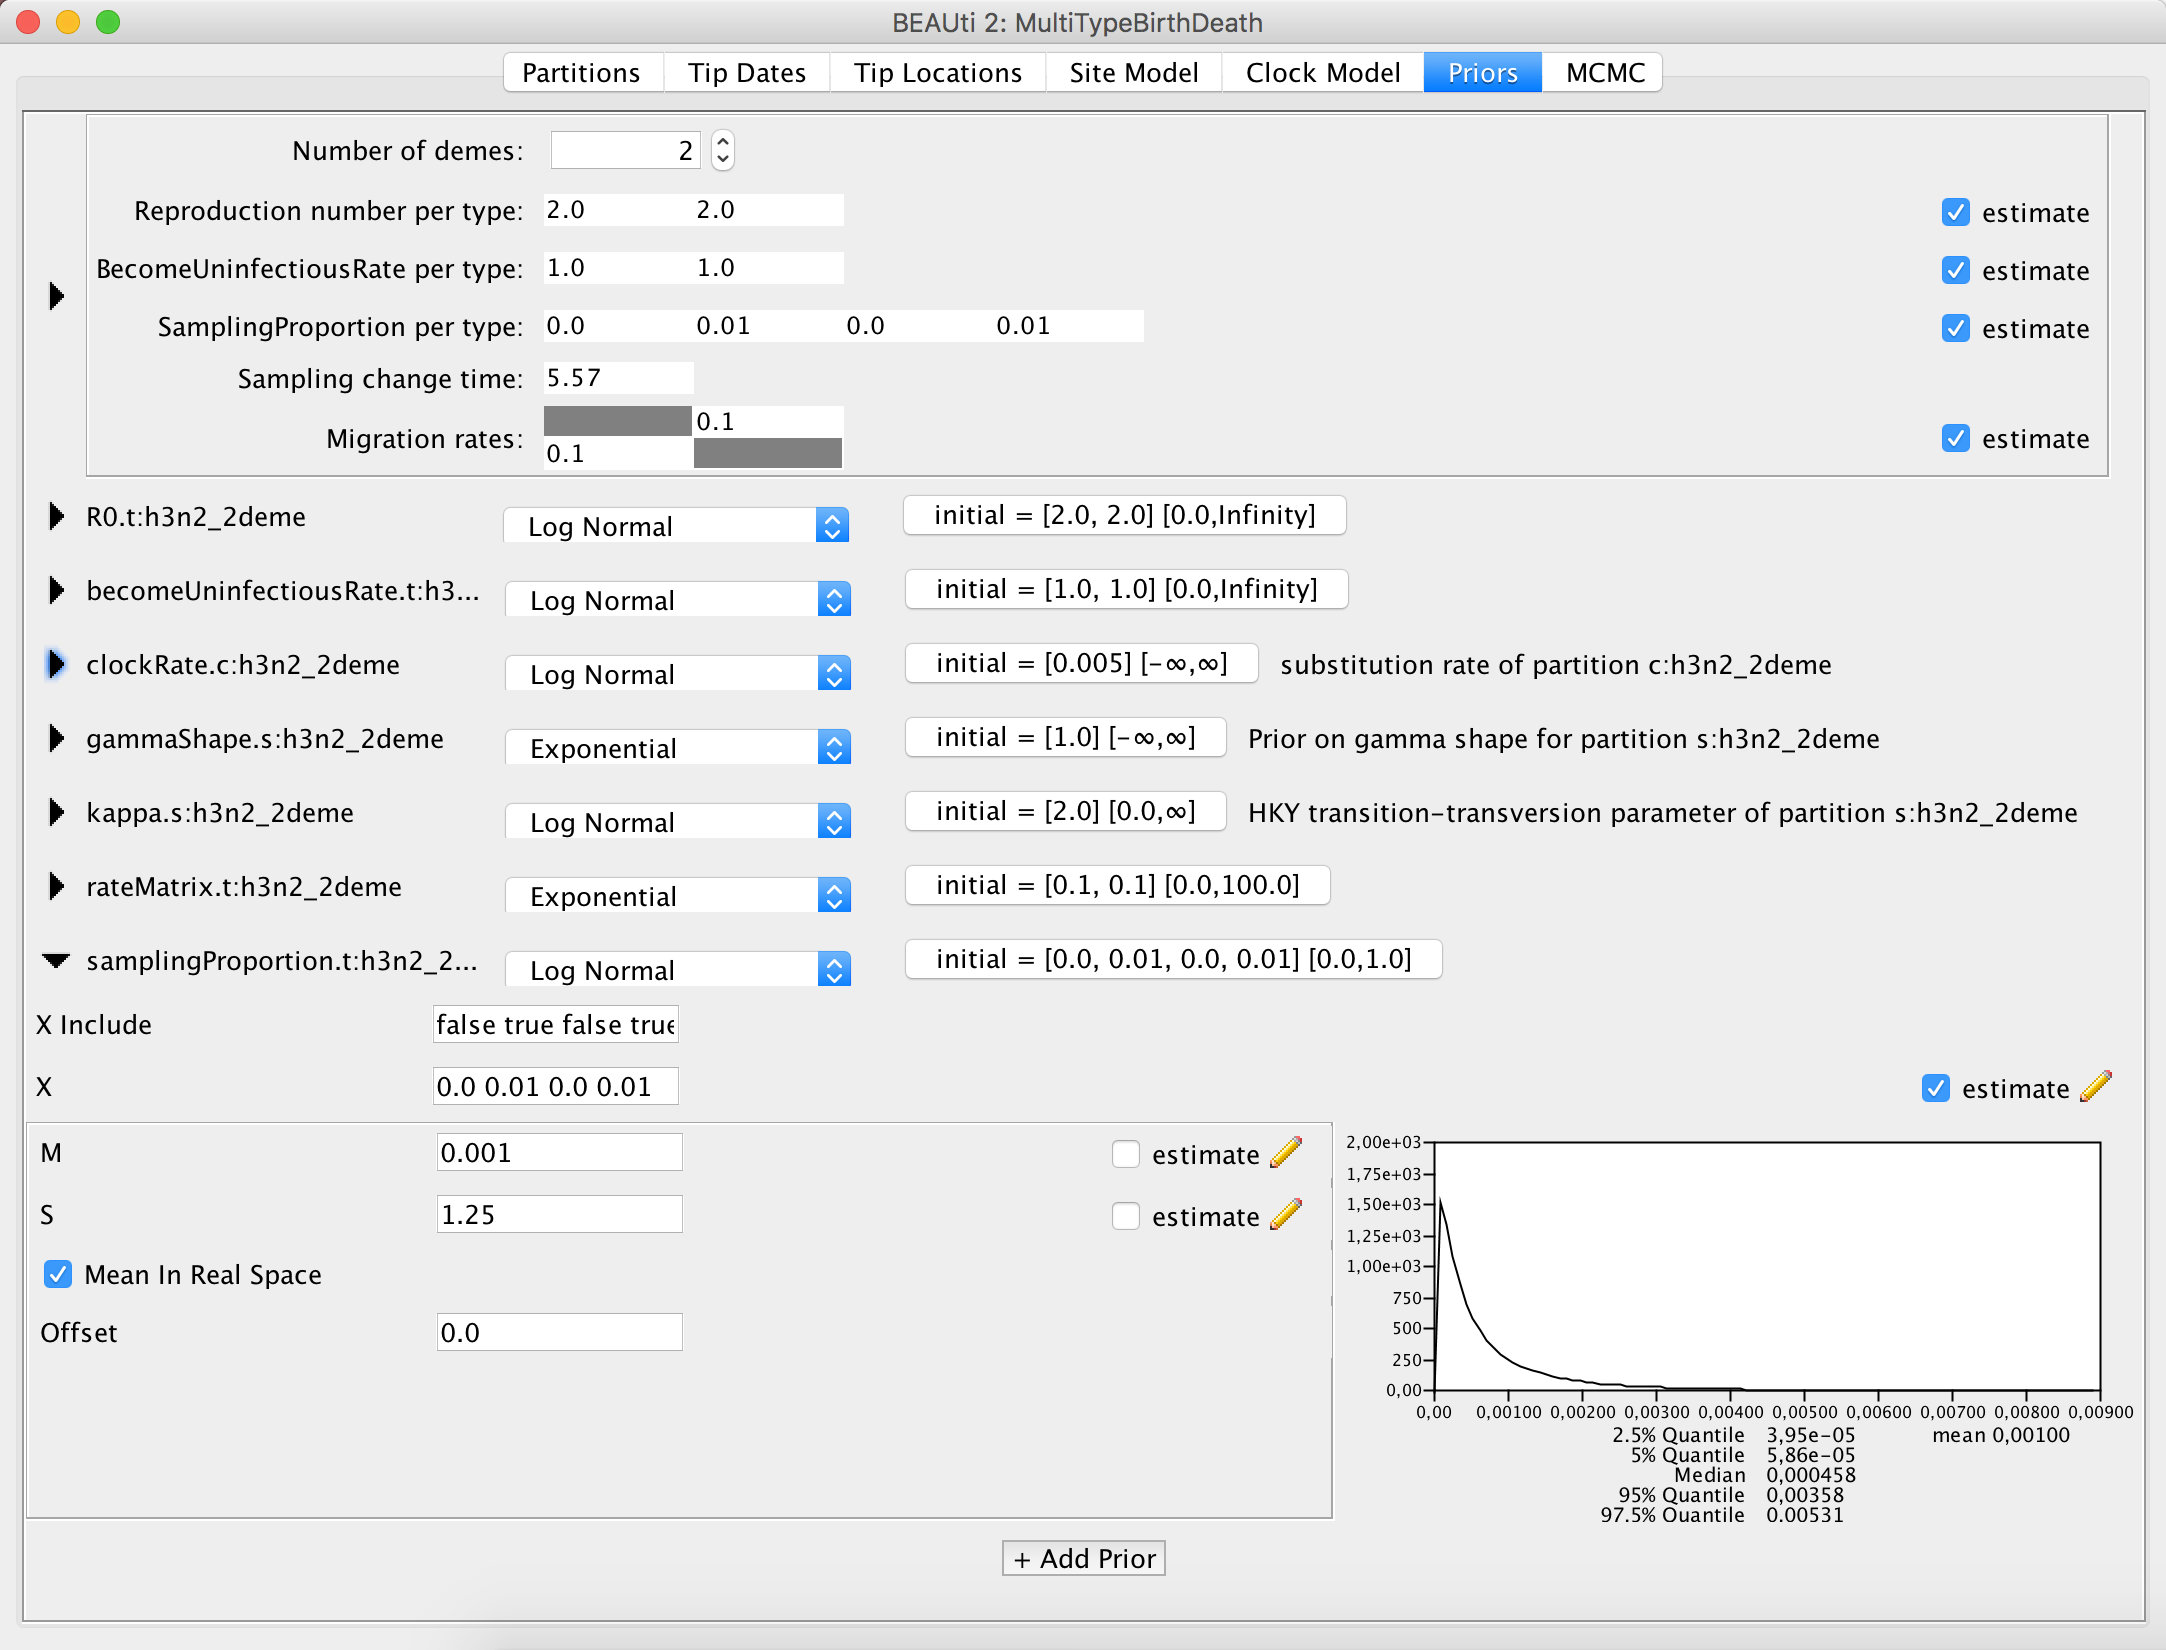
\includegraphics[width=1.000000\textwidth]{figures/15-samplingProportion-prior.png}
    \caption{Set the prior for sampling proportion.}
    \label{fig:samplingProportion-prior}
\end{figure}

For the purpose of this tutorial and given that we know little about the
outbreak in question to set strict priors on the \lstinline!rateMatrix!,
we will leave the other priors on the default values, but feel free to
through them yourself and verify their sensibility.

\subsection{Saving the configuration}\label{saving-the-configuration}

Once you are done with setting all the appropriate parameters, you can
save the configuration file. We will leave the \lstinline!MCMC! panel
parameters as they are by default.

\section{Running the analysis using
BEAST}\label{running-the-analysis-using-beast}

To run the analysis, simply start BEAST 2 in the manner appropriate for
your platform, then select the configuration file you generated in the
last section as the input. Unfortunately, this particular run will take
quite some time to mix, e.g.~on a on a MacBook Pro with 3.1 GHz Intel Core i5
 processor it takes about 3 hours for 10'000'000 samples. 
 Feel free to run it and observe the
results, but for the purpose of finishing the tutorial in a reasonable
time, check out the provided log file to see the results.

\section{Analyzing the results}\label{analyzing-the-results}

The results of the analysis primarily consist of two parts:

\begin{enumerate}
\def\labelenumi{\arabic{enumi}.}

\item
  The parameter log, which is written to the file
  \lstinline!h3n2-bdmm.log!.
\item
  The tree log, which is written to
  \lstinline!h3n2-bdmm.h3n2_2deme.trees!.
\end{enumerate}

In addition, the file \lstinline!h3n2-bdmm.h3n2_2deme.map.trees!
contains the running estimate of the MAP tree as a function of MCMC step
number, while the file \lstinline!h3n2-bdmm.h3n2_2deme.typedNode.trees!
is the TreeAnnotator-compatible file we'll use to assemble a summary
tree.

\subsection{Parameter log file
analysis}\label{parameter-log-file-analysis}

We can use the program
\href{http://tree.bio.ed.ac.uk/software/tracer/}{Tracer} to view the
parameter log file. To do this, start Tracer and then press the
\lstinline!+! button in the top-left hand corner of the window (under
\lstinline!Trace files!). Select the log file for this analysis
(\lstinline!h3n2_2deme.log!) from the file selection dialog box. You can
also simply drag your log file from the file browser to the Tracer
window. The \lstinline!Traces! table will then be populated with
parameters and summary statistics corresponding to our multitype
birth-death analysis. Note that the screen captures below were taken using Tracer 1.6 and may therefore slightly differ from what you see on screen.

Important traces are:

\begin{itemize}
\item
  \lstinline!R0.t:h3n2_2deme1! and \lstinline!R0.t:h3n2_2deme2!: These
  give the effective reproduction numbers for deme 1 (Hong Kong) and 2
  (New Zealand), respectively.
\item
  \lstinline!becomeUninfectiousRate.t:h3n2_deme21! and
  \lstinline!becomeUninfectiousRate.t:h3n2_deme22!: These are the rates
  of recovery for someone with flu in either of the locations.
\item
  \lstinline!rateMatrix.t:h3n2_2deme1! and
  \lstinline!rateMatrix.t:h3n2_2deme2!: These give the (per lineage per
  year) migration rates from deme 1 to 2 and vice versa.
\item
  \lstinline!Tree.t:h3n2_2deme.count_HongKong_to_NewZealand!: these give
  the actual number of ancestral migrations from Hong Kong to New
  Zealand.
\end{itemize}

The tabs at the top-right of the window can be used to display one or
more selected traces in various ways. We can look at the become
uninfectious rate by selecting the
\lstinline!becomeUninfectiousRate.t:h3n2_2deme1! trace (see Figure
\ref{fig:tracer-bUR}). The 95\% HPD for the parameter is quite wide
({[}18.2465, 93.2316{]}), which is most likely due to the fact that we
have very little data, however the mean value is 50.102, which gives us
an infectious period of 7.3 days. Next, selecting the two R0 traces
(\lstinline!R0.t:h3n2_2deme1! and \lstinline!R0.t:h3n2_2deme2!) and
choosing the \lstinline!Marginal prob distribution! panel results in
useful comparison between the sampled population size marginal posterior
distributions (see Figure \ref{fig:tracer-R0}). Looking at the posterior
distributions we can not see any significant difference in R0 between
the two demes. While the distributions are visibly different, they cover
the same parameter range (deme 1 95\% HPD interval {[}0.991, 1.0247{]},
deme 2 95\% HPD interval {[}0.9096, 1.0413{]}), so the values are
indistinguishable through such analysis.

\begin{figure}
    \centering
    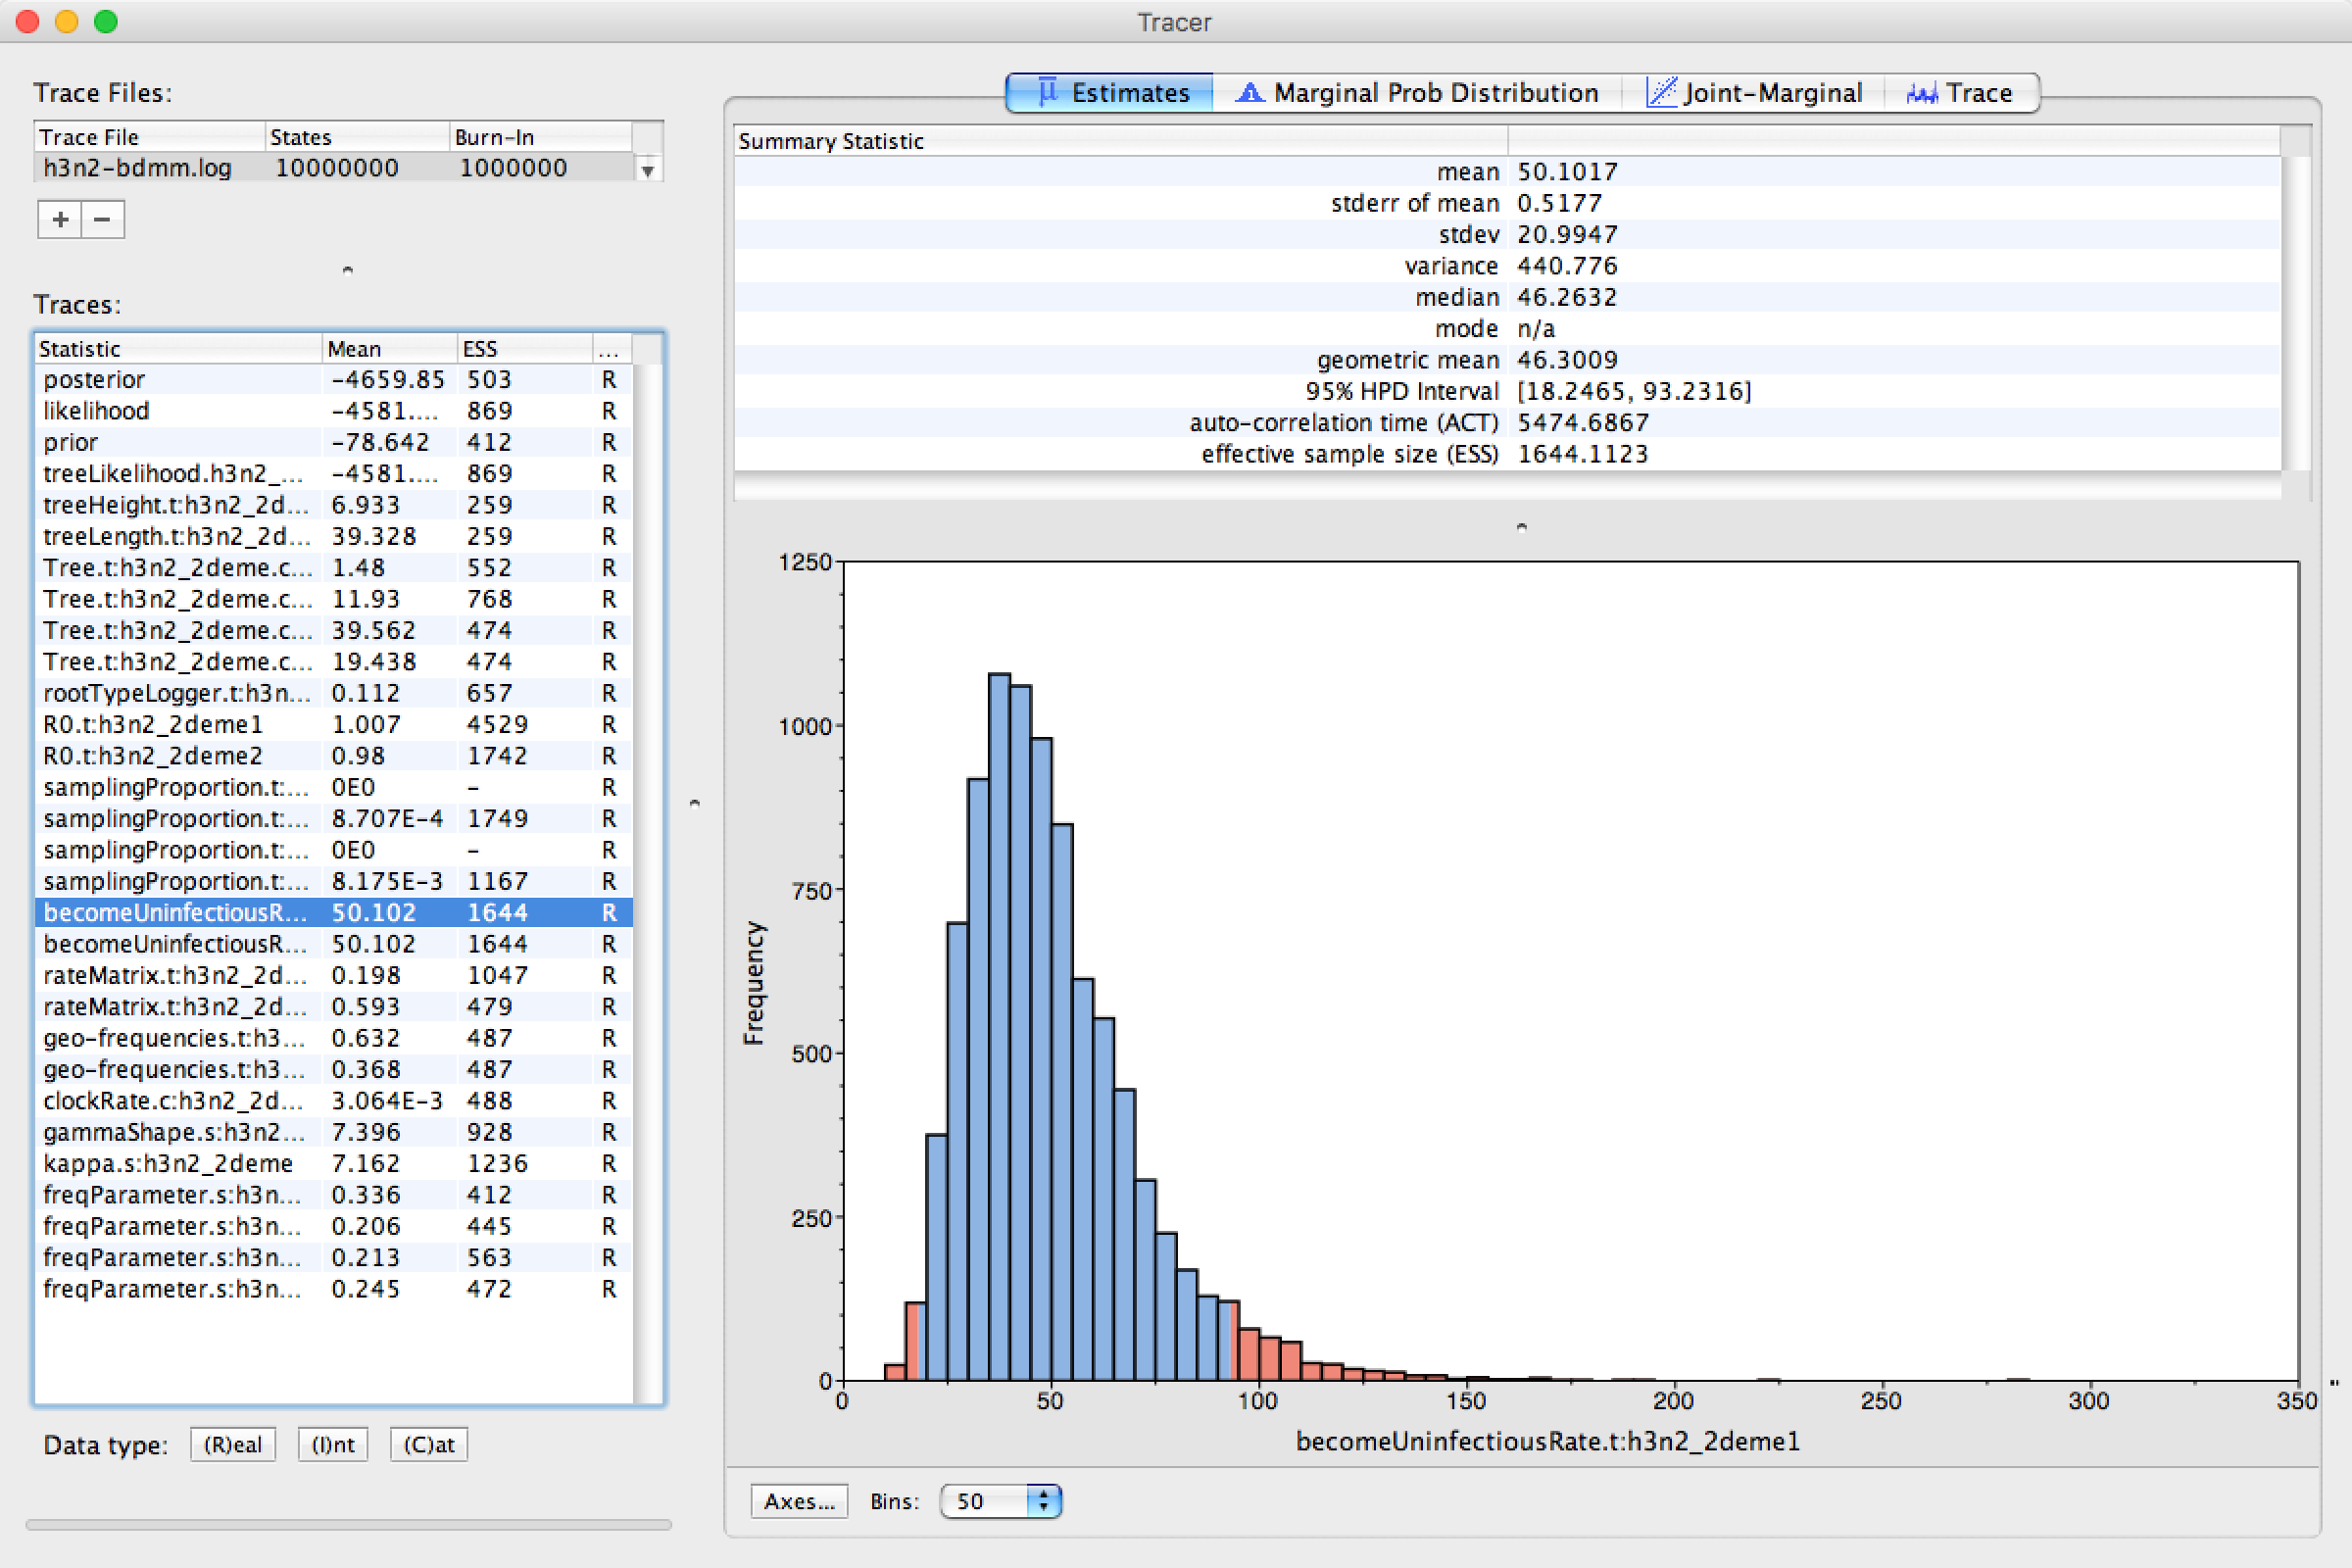
\includegraphics[width=1.000000\textwidth]{figures/16-tracer-bUR.png}
    \caption{Estimated become uninfectious rate marginal posterior.}
    \label{fig:tracer-bUR}
\end{figure}

\begin{figure}
    \centering
    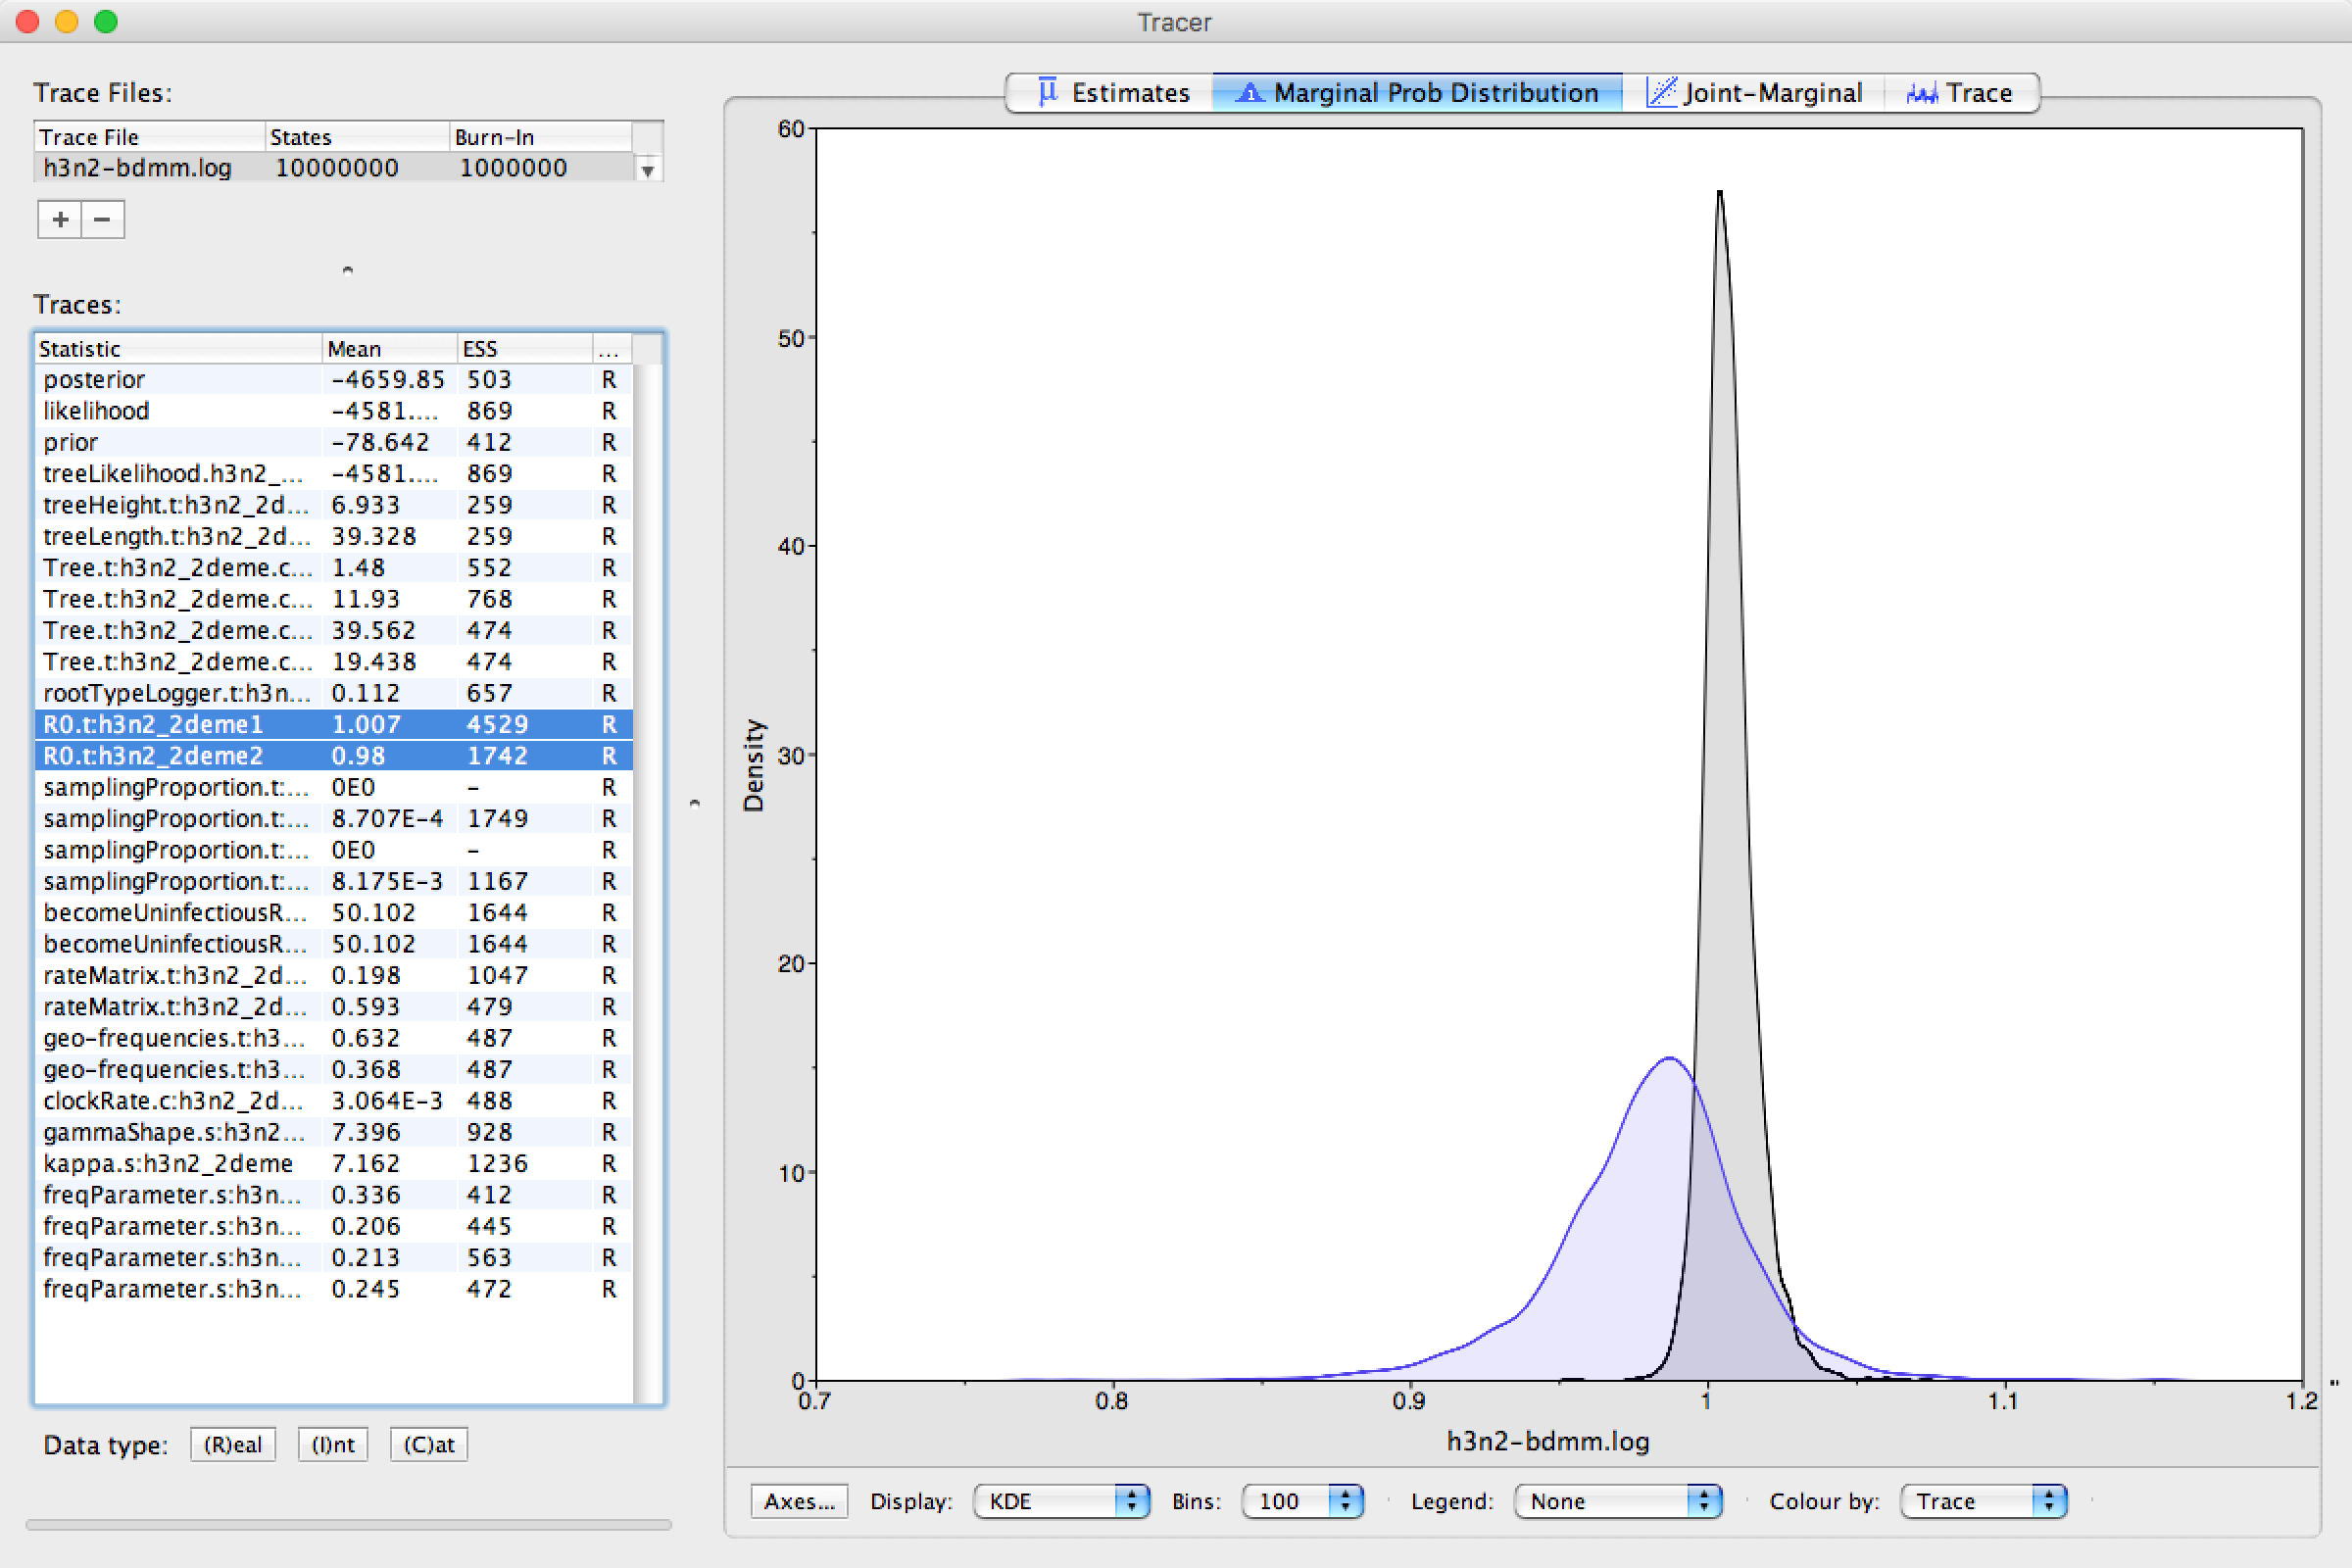
\includegraphics[width=1.000000\textwidth]{figures/17-tracer-R0.png}
    \caption{Estimated R<sub>0</sub> marginal posteriors.}
    \label{fig:tracer-R0}
\end{figure}

In the case of our pre-cooked analysis all the ESS values are greater
than 200 -- the arbitrary threshold for acceptability. However, it might
happen that some values have not yet reached the appropriate ESS in the
runs that you did on your own. If this analysis were part of a serious
study you would want to run the chain for another few million iterations
to improve the ESS values. In BEAST 2, analyses can be resumed -- the
samples you already have will not be wasted.

\subsection{Tree log visualization}\label{tree-log-visualization}

The popular phylogenetic tree visualizer
\href{http://tree.bio.ed.ac.uk/software/figtree/}{FigTree} can be used
to visualize the sampled trees. However, Figtree can be quite slow with
MultiTypeTree log files, so for this tutorial we suggest using
\href{https://icytree.org/}{IcyTree} to view tree log files. IcyTree is
a tree viewer that runs in a web browser, which runs best under recent
versions of \href{http://www.google.com/chrome}{Google Chrome} and
\href{https://www.mozilla.org/en-US/firefox/}{Mozilla Firefox} (in that
order).

To view MultiTypeTree log files using IcyTree, simply navigate to the
IcyTree web page, select \lstinline!Load from file! from the
\lstinline!File! menu, then select the
\lstinline!h3n2-bdmm.h3n2_2deme.trees! tree log file using the file
selection dialog. Alternatively, you can simply drag the log file into
your browser window. Once the file is loaded you will see the first tree
it contains. In order to select a different tree, hover the mouse
pointer over the box in the lower-left corner of the window. This box
will expand to a small dialog containing buttons allowing you to
navigate between trees. The \lstinline!<! and \lstinline!>! buttons move
in steps of 1 tree, while \lstinline!<<! and \lstinline!>>! move 10\% of
the tree file. You can also directly enter the index of a tree.

Initially the tree edges will be uncoloured. To colour the edges
according to the edge type (this is the strain location in our case),
navigate to \lstinline!Style > Colour edges by! and select
\lstinline!type!. A legend and axis can be added by choosing
\lstinline!Display legend! and \lstinline!Axis > Age! from the same
menu. You can browse the trees from your posterior sample (example of
the trees you can see in Figure \ref{fig:icyTree-trees}) to look at the
traits they share, however in general we need some sort of a summary to
be able to draw conclusions from our tree sample.

\begin{figure}
    \centering
    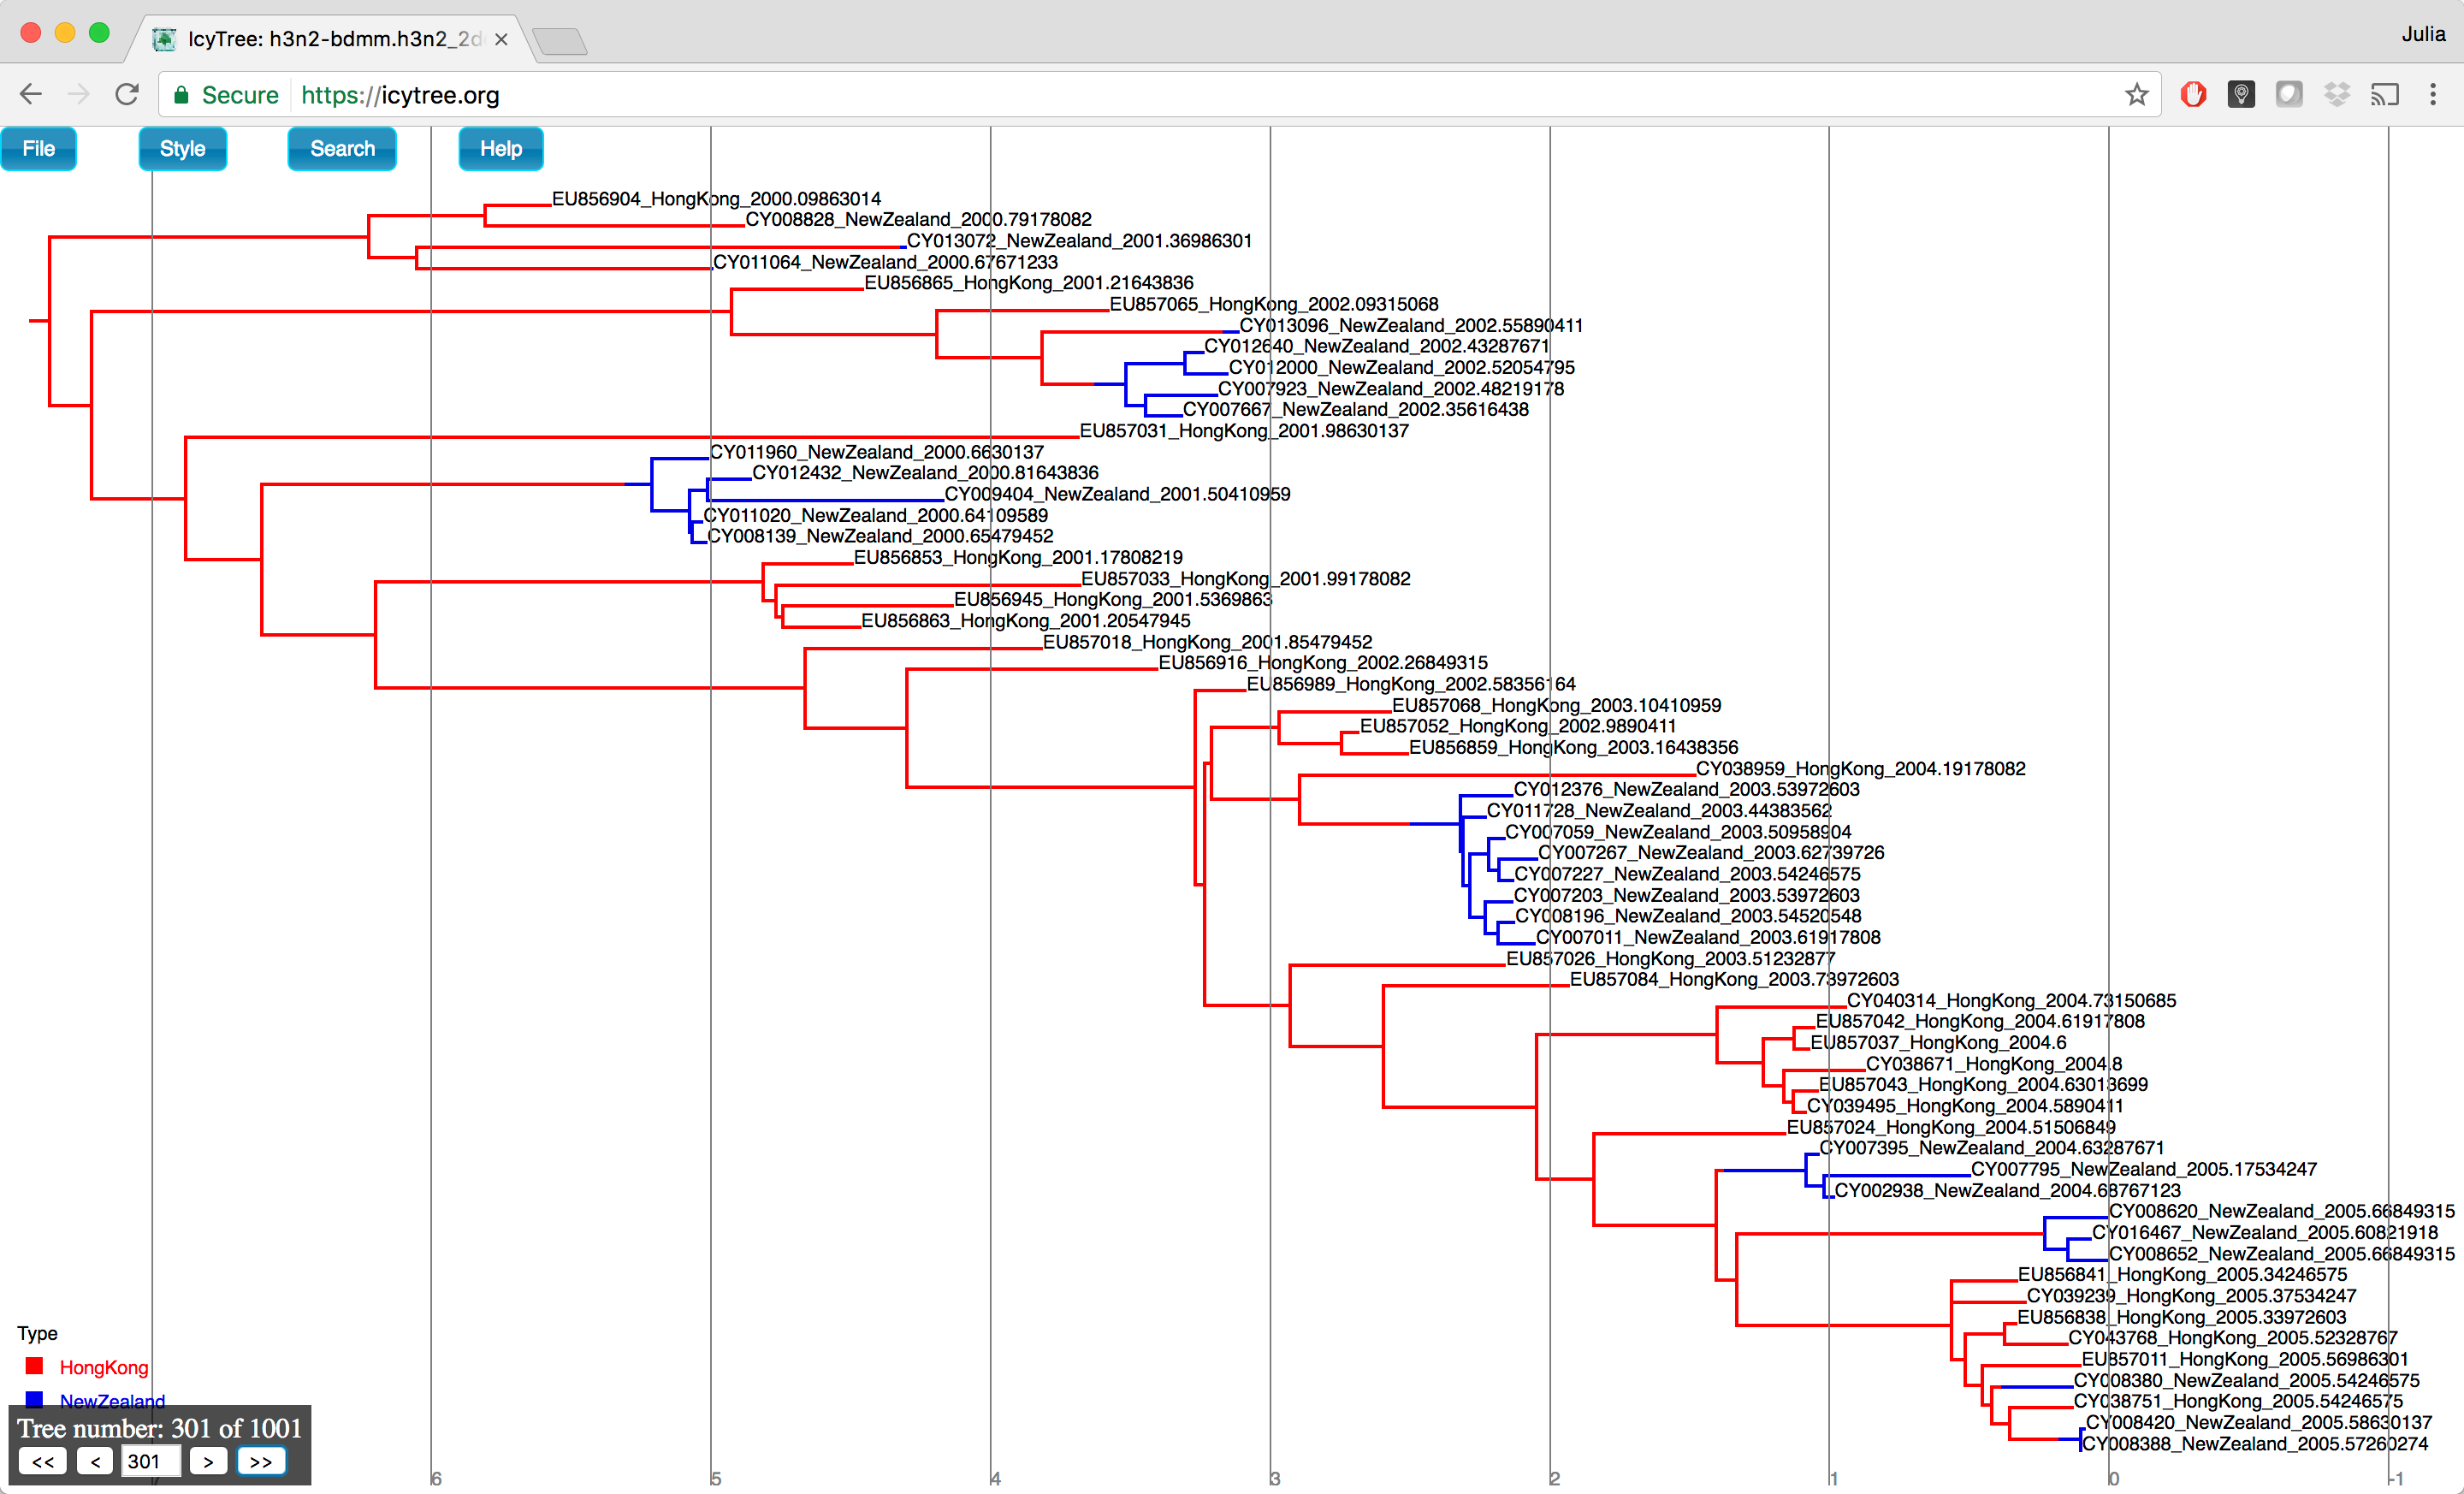
\includegraphics[width=1.000000\textwidth]{figures/18-icyTree-trees.png}
    \caption{An example of a sampled multi-type tree in IcyTree.}
    \label{fig:icyTree-trees}
\end{figure}

One way of summarising is done by the special \lstinline!MultiTypeTree!
log, which logs the running estimates of the maximum a posteriori
multi-type tree over the course of the analysis. In our case it is the
\lstinline!h3n2-bdmm.h3n2_2deme.map.trees! file. You can see the last
tree from this file, which represents our sampled estimate of the MAP
multi-type tree, in Figure \ref{fig:icyTree-MAP}.

\begin{figure}
    \centering
    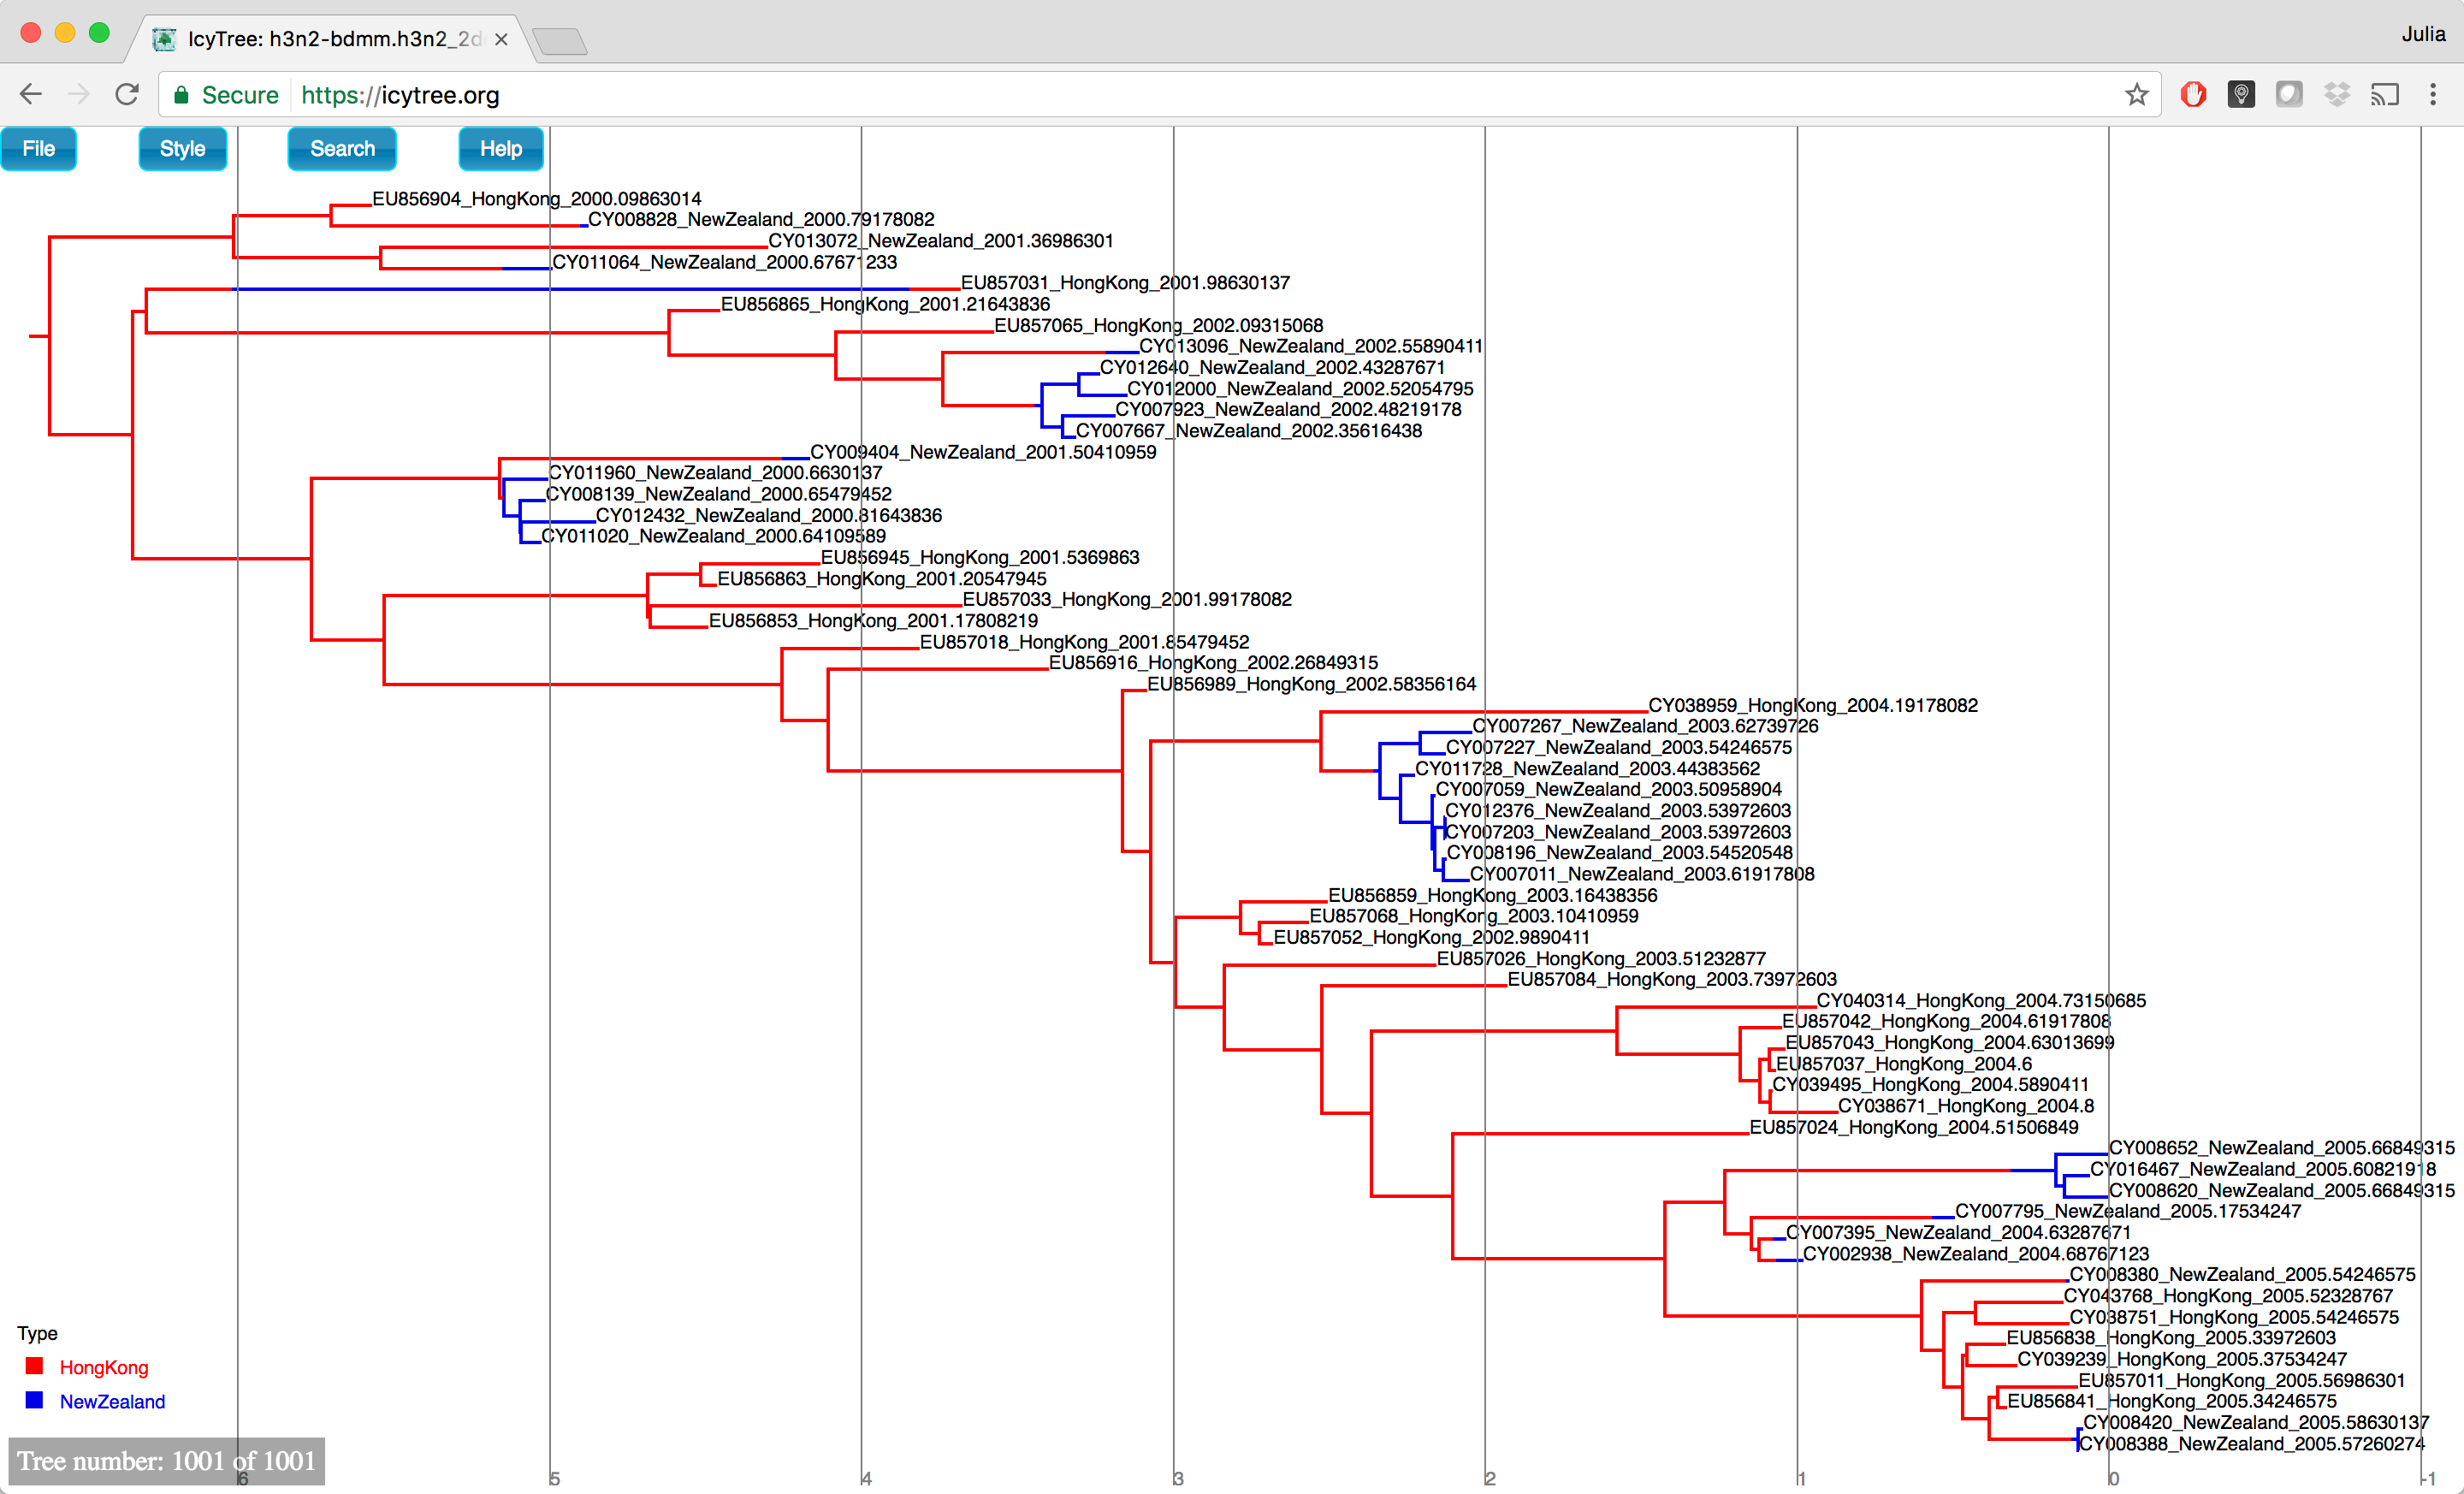
\includegraphics[width=1.000000\textwidth]{figures/19-icyTree-MAP.png}
    \caption{The final MAP multi-type tree in IcyTree.}
    \label{fig:icyTree-MAP}
\end{figure}

\subsection{\texorpdfstring{Producing a summary tree using
\texttt{TreeAnnotator}}{Producing a summary tree using TreeAnnotator}}\label{producing-a-summary-tree-using-treeannotator}

While it is tempting to view the MAP tree shown above as the primary
result of the phylogenetic side of our analysis it is very important to
remember that this is only a point estimate and says nothing about the
uncertainty present in the result. This is an important drawback, as we
have done a full Bayesian analysis and have access to a large number of
samples from the full posterior in the tree log files. The MAP tree
discards almost all of this information.

We can make better use of our raw analysis results by using the
\lstinline!TreeAnnotator! program which is distributed with BEAST2 to
analyze the sample of trees which was produced by our MCMC run. To do
this, simply start \lstinline!TreeAnnotator! and select the
\lstinline!h3n2-bdmm.h3n2_2deme.typedNode.trees! tree file as the input
file and \lstinline!h3n2-bdmm.h3n2_2deme.summary.trees! as the output
file. We will set the \lstinline!Burnin percentage! to 10, the
\lstinline!Target tree type! to the
\lstinline!Maximum clade credibility tree! (default) and for the
\lstinline!Node heights! we would like to have \lstinline!Mean heights!.
The setup can be seen in Figure \ref{fig:TreeAnnotator-setup}.

\begin{figure}
    \centering
    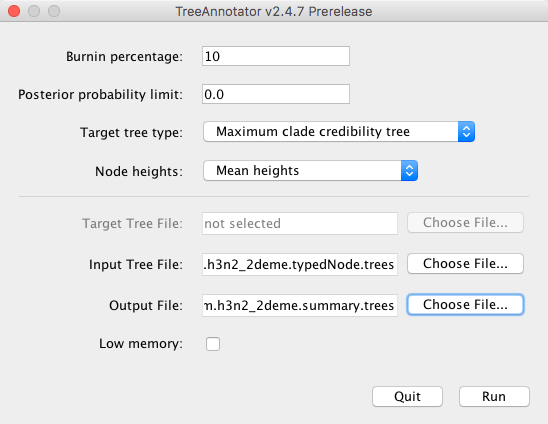
\includegraphics[width=0.750000\textwidth]{figures/20-TreeAnnotator-setup.png}
    \caption{Use TreeAnnotator to produce a summary tree.}
    \label{fig:TreeAnnotator-setup}
\end{figure}

Pressing the \lstinline!Run! button will produce an annotated summary
tree.

To visualize this tree, open IcyTree once more (maybe open it in a new
browser tab), choose \lstinline!File > Open!, then select the file
\lstinline!h3n2_2deme.h3n2_2deme.summary.tree! using the file selection
dialog. Follow the instructions provided above to colour the tree by the
\lstinline!type! attribute and add the legend and time axis. In
addition, open the \lstinline!Style! menu and select
\lstinline!Node height error bars > height_95%_HPD! to add error bars to
the internal node heights. Finally, open the \lstinline!Style! menu and
select \lstinline!Relative edge width > type.prob!. This makes the edges become increasingly thinner as the posterior probability for the displayed branch decreases.

Once these style preferences have been set, you should see something
similar to the tree shown in Figure \ref{fig:icyTree-summary}.

\begin{figure}
    \centering
    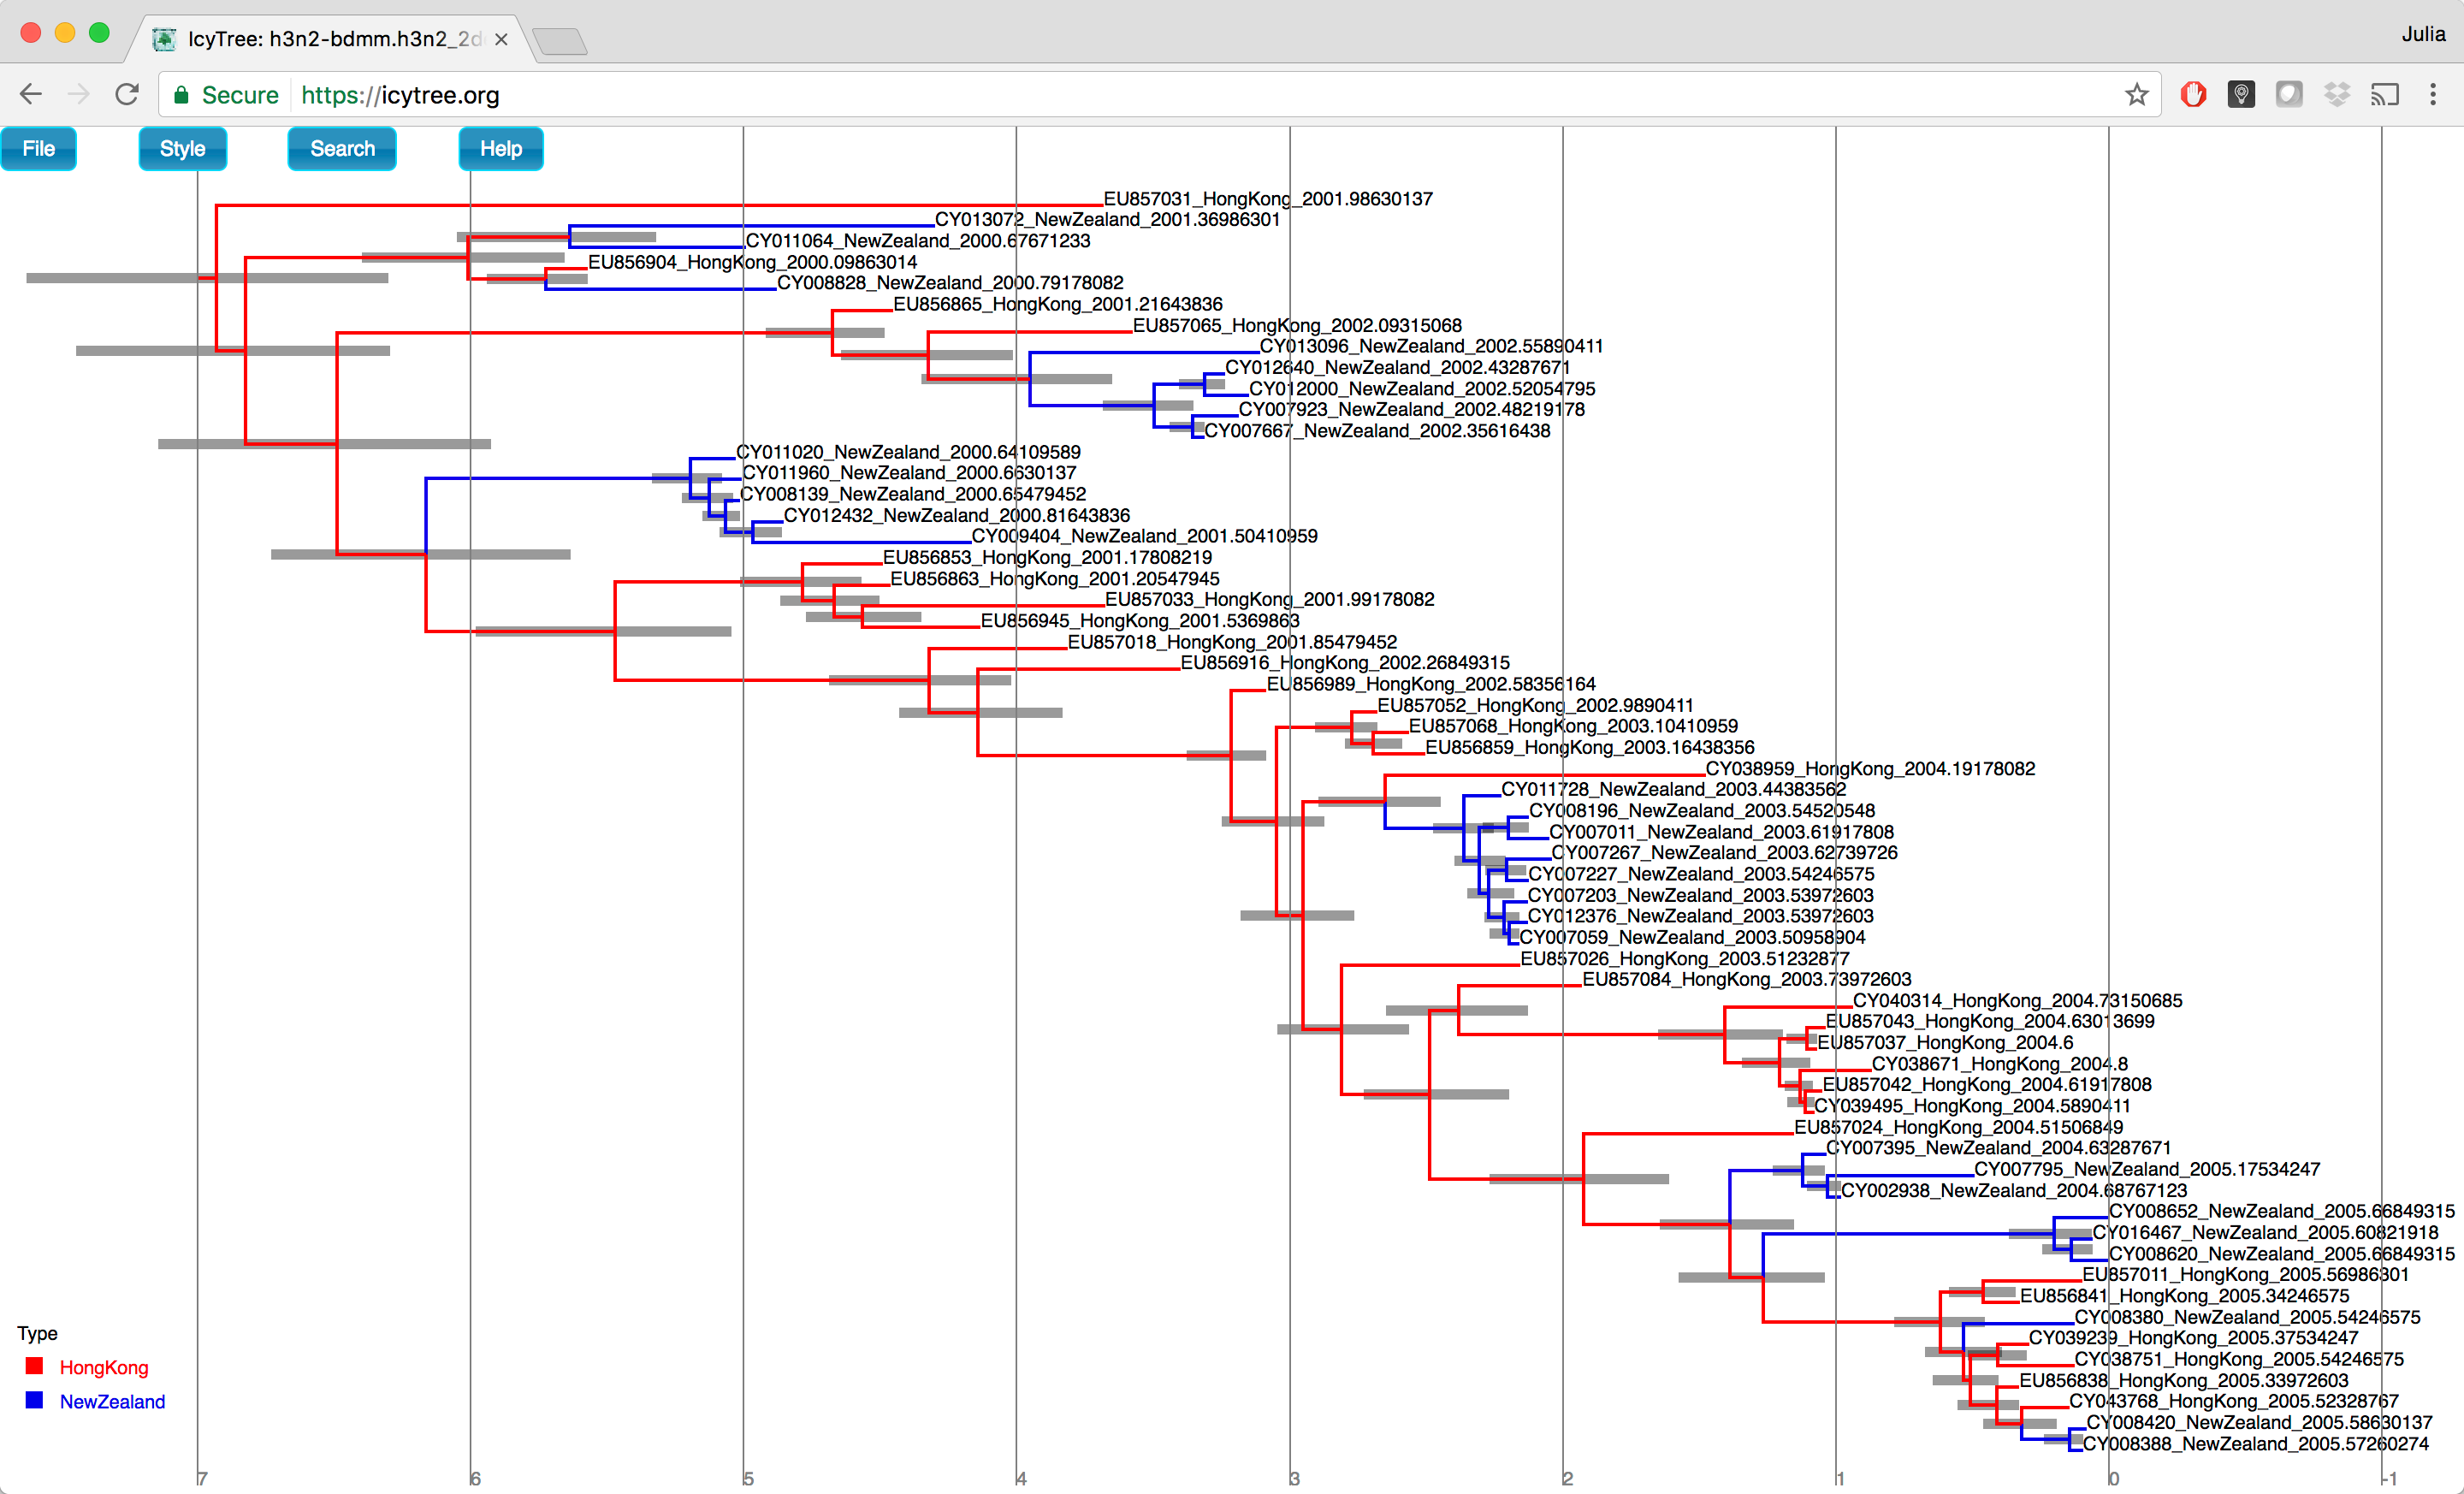
\includegraphics[width=1.000000\textwidth]{figures/21-icyTree-summary.png}
    \caption{The summary tree in IcyTree.}
    \label{fig:icyTree-summary}
\end{figure}

Here we have a full consensus tree annotated by the locations at
coalescence nodes and showing node height uncertainty, with the
width/transparency of the edges representing how certain we can be of
the location estimate at each point on the tree. This is a much more
comprehensive summary of the phylogenetic side of our analysis. One
thing to pay attention to here is that the most probable root location
in the summary tree is Hong Kong (under our model which assumes that
only Hong Kong and New Zealand exist). Hovering the mouse cursor over
the tiny edge above the root will bring up a table in which posterior
probability of the displayed root location (\lstinline!type.prob!) can
be seen. In this analysis we see that it is about 88.8\%. The analysis
therefore strongly supports a Hong Kong origin over a New Zealand origin
for this flu sample.

\section{Acknowledgment}\label{acknowledgment}

The content of this tutorial is based on the
\href{https://github.com/CompEvol/MultiTypeTree/wiki/Beginner's-Tutorial-(short-version)}{Structured
Coalescent tutorial} by Tim Vaughan.

\section{Useful Links}\label{useful-links}

\begin{itemize}

\item
  \href{http://www.beast2.org/book.html}{Bayesian Evolutionary Analysis
  with BEAST 2} \citep{BEAST2book2014}
\item
  \href{https://github.com/denisekuehnert/bdmm}{Multi-type birth-death
  process package} \citep{Kuhnert2016}
\item
  BEAST 2 website and documentation: \url{http://www.beast2.org/}
\end{itemize}



%%%%%%%%%%%%%%%%%%%%%%%
% Tutorial disclaimer %
%%%%%%%%%%%%%%%%%%%%%%%
% Please do not change the license
% Add the author names and relevant links
% Add any other aknowledgments here
\href{http://creativecommons.org/licenses/by/4.0/}{\includegraphics[scale=0.8]{figures/ccby.pdf}} This tutorial was written by Denise Kühnert and Jūlija Pečerska for \href{https://taming-the-beast.github.io}{Taming the BEAST} and is licensed under a \href{http://creativecommons.org/licenses/by/4.0/}{Creative Commons Attribution 4.0 International License}. 


%%%%%%%%%%%%%%%%%%%%
% Do NOT edit this %
%%%%%%%%%%%%%%%%%%%%
Version dated: \today



\newpage 
%%%%%%%%%%%%%%%%
%  REFERENCES  %
%%%%%%%%%%%%%%%%

\printbibliography[heading=relevref]


\end{document}